%%%%%%%%%%%%%%%%%%%%%%%%%%%%%%%%%%%%%%%%%%%%%%%%%%%%%%%
%% Engineer & Master Thesis, LaTeX Template          %%
%% Copyleft by Piotr Woźniak & Artur M. Brodzki      %%
%% Faculty of Electronics and Information Technology %%
%% Warsaw University of Technology, Warsaw, 2019     %%
%%%%%%%%%%%%%%%%%%%%%%%%%%%%%%%%%%%%%%%%%%%%%%%%%%%%%%%

\documentclass[
    left=2.5cm,         % Sadly, generic margin parameter
    right=2.5cm,        % doesnt't work, as it is
    top=2.5cm,          % superseded by more specific
    bottom=3cm,         % left...bottom parameters.
    bindingoffset=6mm,  % Optional binding offset.
    nohyphenation=true % You may turn off hyphenation, if don't like. =false
]{eiti/eiti-thesis} % bazuje na clasie mwart

\nocite{*}

\usepackage[
    backend=bibtex,
]{biblatex}
\usepackage{csquotes}
\usepackage{hyperref}
\usepackage{algpseudocode}
\usepackage{algorithm}
\usepackage{url}

\langpol % Dla języka angielskiego mamy \langeng
\graphicspath{{img/}}             % Katalog z obrazkami.
\bibliography{bib-mendeley.bib,bib-other.bib} % Plik .bib z bibliografią`'

\makeatletter
\xpatchcmd\lst@MakeCaption{\protect\numberline{\thelstlisting}\lst@@caption}{\protect\numberline{\thelstlisting.}\lst@@caption}{}{}
%\makeatother
%\makeatletter
%\xpatchcmd{\LT@c@ption}{\protect\numberline{\thetable}}{\protect\numberline.{. \thetable . }}{}{}
\makeatother

\begin{document}

%--------------------------------------
% Strona tytułowa
%--------------------------------------
\RaportThesis
\instytut{Cyberbezpieczeństwa}
\kierunek{Telekomunikacja}
\specjalnosc{Techniki Teleinformatyczne}
\title{
    Akceleracja sprzętowa kryptoanalizy algorytmów kryptograficznych
}
\engtitle{ % Tytuł po angielsku do angielskiego streszczenia
    Hardware acceleration of cryptoanalysis of cryptograhpic algorithms
}
\author{Andrzej Tłomak}
\album{311450}
\promotor{dr. hab. inż. Mariusz Rawski}
\date{\the\year}
\maketitle

%--------------------------------------
% Streszczenie po polsku
%--------------------------------------
\streszczenie
Cel pracy
\slowakluczowe Krzywe eliptyczne, Kryptografia, Kryptoanaliza, CUDA, Algorytm~rho~Pollard'a
\newpage

%--------------------------------------
% Streszczenie po angielsku
%--------------------------------------
\abstract
The objective of this phase included a review of the literature describing the current State-of-Art \
in cryptoanalysis of systems \
based on Elliptic curves in Finite Fields. It involved getting deeper knowledge of theory
and mathematical fundation of Elliptic curves as well as setting up an environment
to develop implementation utillizing CUDA technology.
\keywords Elliptic curves, Cryptography, Cryptoanalysis, CUDA, FPGA, rho~Pollard~algorithm
\newpage

%--------------------------------------
% Oświadczenie o autorstwie
%--------------------------------------
\makeauthorship
\blankpage

%--------------------------------------
% Spis treści
%--------------------------------------
%\thispagestyle{empty}
\tableofcontents
%\blankpage

% Listing ustawienia
% \lstset{
%     language=C,                     % Use 'C' for CUDA as a base
%     basicstyle=\ttfamily\small,     % Font size and type
%     keywordstyle=\color{blue},      % Keywords in blue
%     commentstyle=\color{green},     % Comments in green
%     stringstyle=\color{red},        % Strings in red
%     frame=single,                   % Frame around the code
%     numbers=left,                   % Add line numbers on the left
%     numberstyle=\tiny,              % Line number font size
%     stepnumber=1,                   % Line number increment
%     tabsize=4,                      % Set tab size
%     breaklines=true,                % Enable line breaking
%     showspaces=false,               % Don't show spaces
%     showstringspaces=false,         % Don't show spaces in strings
%     captionpos=b,                   % Caption position at bottom
% }

%--------------------------------------
% Rozdziały
%--------------------------------------
\newpage
\section{Wprowadzenie}

Wraz z rosnącą potrzebą zapewnienia poufności i integralności danych w systemach
informatycznych, kryptografia stała się jednym z filarów współczesnych rozwiązań
bezpieczeństwa. Kryptografia oparta na krzywych eliptycznych \textbf{ECC} ( \textit{Elliptic Curve Cryptography}) jest
obecnie jednym z najważniejszych standardów w tej dziedzinie, oferując wysoki
poziom bezpieczeństwa przy znacznie mniejszych rozmiarach kluczy w porównaniu
do tradycyjnych algorytmów, takich jak RSA \cite[]{Ao2016,Barker2016}.
Z tego powodu ECC znajduje szerokie zastosowanie w systemach o ograniczonych zasobach,
urządzeniach IoT ( \textit{Internet of Things}) czy urządzeniach mobilnych \cite[]{Thakur2022,Hammi2020}.

Bezpieczeństwo ECC opiera się na trudności rozwiązania problemu logarytmu
dyskretnego na krzywych eliptycznych. Jest to problem matematyczny, który w
praktyce nie ma efektywnego rozwiązania w rozsądnym czasie przy użyciu
współczesnych metod obliczeniowych. Do tej pory nie opracowano algorytmu
zdolnego rozwiązać ten problem w czasie podwykładniczym na komputerach klasycznych, dlatego
kryptoanaliza ECC wymaga dużych zasobów obliczeniowych \cite{Menezes2001}.
Z tego powodu, często wykorzystywane w tej roli są układy GPU \cite[]{Boss2015,Panetta2017,Bernstein2012},
FPGA \cite[]{Wenger2014,Mane2011,FPGA2008,Majkowski2008}
czy nawet konsole dla graczy \cite{Bos2010}.

Gwałtowny rozwój kart graficznych \textbf{GPU} ( \textit{Graphic Processing Unit})
oraz technologii \textbf{CUDA} ( \textit{Compute Unified Device Architecture}) znacznie zwiększył możliwości
przeprowadzania takich analiz. Choć rozwój ten był w dużej mierze napędzany
zapotrzebowaniem związanym z uczeniem maszynowym, jego zastosowanie w
innych dziedzinach, takich jak kryptoanaliza jest równie istotny.

Karty graficzne, dzięki architekturze zoptymalizowanej do równoległych obliczeń,
stały się narzędziem o kluczowym znaczeniu w dziedzinach wymagających intensywnego
przetwarzania danych. Platforma CUDA, opracowana przez firmę NVIDIA, umożliwia
wykorzystanie mocy obliczeniowej GPU do realizacji zadań takich jak
implementacja algorytmów kryptograficznych oraz analiza ich odporności na ataki.
CUDA pozwala na masywnie równoległe przetwarzanie danych, co ma kluczowe znaczenie
w implementacji algorytmu Rho Pollard'a, który w wersji równoległej, pozwala na efektywne
wykorzystanie możliwości GPU.

Chociaż GPU nie oferują wydajności i efektywności energetycznej 
porównywalnej z dedykowanymi układami, takimi jak FPGA czy ASIC, ich dostępność 
i stosunkowo niski koszt czyni je atrakcyjnym wyborem do obliczeń kryptograficznych. 
W obliczu rosnącej mocy obliczeniowej GPU oraz ich szerokiej dostępności, ciągła 
analiza odporności algorytmów kryptograficznych na ataki staje się jeszcze 
ważniejszym elementem ich rozwoju.

\subsection{Cel pracy}
Celem tej pracy jest realizacja systemu korzystającego z koprocesora GPU,
w celu przyśpieszenia obliczeń przy
rozwiązywaniu problemu logarytmu dyskretnego.
Implementacja została zoptymalizowana i dostosowana do obliczenia logarytmu
dyskretnego na krzywej eliptycznej ECCp-79, zaproponowanej w wyzwaniu \textit{The Certicom ECC Challenge} \cite{certicom-challange}.
\par
Głównymi elementami stworzonego systemu
jest program klienta wykonującego część algorytmu Rho Pollard'a na karcie graficznej Nvidia
z wykorzystaniem technologii CUDA i języka programowania CUDA C++,
oraz program serwera działający na CPU, odpowiedzialny za zarządzanie klientami i zbieranie wyników.
 Wyniki implementacji zostały porównane z innymi pracami
których celem była kryptoanaliza ECC z wykorzystaniem akceleracji sprzętowej.
\newpage
\section{Wstęp teoretyczny}

\subsection{Procesor graficzny}
Procesory graficzne są specjalnym rodzajem procesorów,
pierwotnie stworzonych do akceleracji obliczeń graficznych.
Obliczenia te charakteryzują się dużą liczbą względnie prostych, podobnych operacji,
które mogą być przeprowadzone równolegle.
Taki model obliczeń nosi nazwę \textbf{SIMD} ( \textit{Single Instruction Multiple Data})
i oznacza równoległe wykonywanie tej samej operacji dla wielu różnych danych wejściowych.
Współczesne karty graficzne są zaprojektowanie do wykorzystania
ich możliwości równoległych obliczeń w znacznie szerszym obszarze niż
pierwotny cel akceleracji grafiki komputerowej.
Technologie \textit{OpenCL} oraz \textit{CUDA} umożliwiają
programowanie GPU w
dziedzinach takich jak obliczenia naukowe, machine learning czy kryptografia.

\par
W pracy, w celu przeprowadzenia ataku na krzywą eliptyczną, wykorzystano
algorytm \textit{Rho Pollard'a}, który z niewielkimi modyfikacjami można bardzo skutecznie wykonywać
równolegle. Z tego powodu wykorzystanie GPU do kryptoanalizy, pozwala znacznie przyśpieszyć czas
obliczeń. W celu stworzenia programu na GPU użyto technologii Nvidia CUDA, głównie ze względu
na znacznie lepiej rozwinięty ekosystem oraz dostępność materiałów w internecie.
Standard OpenCL w przeciwieństwie do CUDA, jest tworzony na zasadach \textit{open-source} oraz może zostać
wykorzystany do programowania kart graficznych innych producentów. Niestety jest zauważalnie
gorzej wspierany w przypadku kart graficznych Nvidia.
\par
\subsubsection{Model programowania CUDA}
Program napisany w CUDA, składa się z jednego lub więcej
\textit{kernel'i} - funkcji programu, która będzie się wykonywać równolegle na GPU, na każdym z uruchomionych wątków.
Wątki są grupowane w \textit{bloki}, które mogą się składać z 1 do 1024 wątków w przypadku \textit{CUDA 7.5} \cite{CudaDeveloper}.
Następnie bloki są uruchamiane na dostępnych jednostkach \textbf{SM} ( \textit{streaming multiprocessor}).
Karty graficzne Nvidia składają się zazwyczaj z kilkunastu SM, które mogą równocześnie uruchomić wiele
bloków, co pozwala na równoczesne wykonywanie kilkuset wątków.
Wątki w ramach jednego bloku dzielą pamięć współdzieloną \textit{shared memory} oraz wykonują się równocześnie.
Możliwe jest uruchomienie znacznie większej ilości bloków, niż może się jednocześnie wykonywać na dostępnych SM.
W takiej sytuacji niektóre bloki będą oczekiwać na wolne zasoby aż poprzednie nie zakończą pracy.
Dodatkowo, wątki w ramach bloku wykonują tą samą instrukcję w grupach po 32,
nazywanych \textit{warp'ami}.
W przypadku architektury SIMD ważne jest unikanie długich segmentów
warunkowych, ponieważ skutkuje to sekwencyjnymi obliczeniami.
W sytuacji gdy następuje rozgałęzienie kodu - \textit{branching},
część wątków w warp'ie musi czekać na pozostałe, skutkując sekwencyjnym wykonywaniem kodu.
Jest to szczególnie istotne dla wydajności działania programu na GPU \cite{CudaDeveloper}.
\subsubsection{Hierarchia pamięci}
Kolejnym ważnym elementem który mocno wpływa na wydajność
programu, jest odpowiedni dostęp do pamięci.
Tak samo jak w zwykłym procesorze, GPU ma kilka warstw
pamięci, które różnią się rozmiarem oraz czasem dostępu.
W CUDA można wyróżnić 3 najważniejsze warstwy pamięci:
\begin{itemize}
    \item Rejestry - najszybszy rodzaj pamięci, dostępny w ramach pojedynczego wątku.
          Ilość rejestrów dla każdego wątku jest jednak mocno ograniczona w przypadku
          uruchomienia wielu wątków równocześnie. Jeżeli program używa wiecej rejestrów niż jest dostępne,
          może wystąpić \textit{register spilling}, który wprowadza znaczne opóźnienia.
    \item \textit{Shared memory} - szybka pamięć współdzielona, która jest wspólna dla wątków w danym bloku. Jest ona ograniczona
          przez ilość pamięci w SM. Na karcie graficznej z CUDA 7.5 jej rozmiar wynosi 64 KB \cite{CudaDeveloper}.
          Stosowana jest w przypadku, gdy wiele wątków musi się ze sobą komunikować lub w celu cache'owania danych
          i ograniczenia dostępu do znacznie wolniejszej pamięci globalnej.
          Zbyt duży rozmiar wykorzystywanej pamięci współdzielonej ogranicza ilość bloków które mogą jednocześnie się
          wykonywać na jednym SM.
    \item \textit{Global memory} - pamięć globalna DRAM, najwolniejsza oraz największa ze wszystkich warstw. Wykorzystywana głównie w celu
          komunikacji karty graficznej z procesorem, w celu przesyłania danych do obliczeń oraz zapisu wyników.
\end{itemize}
Dostępne są również dodatkowe rodzaje takie jak \textit{texture memory} oraz \textit{constant memory},
które różnią się optymalnym sposobem dostępu, jednak nie są wykorzystywane w tej pracy.

\subsection{Krzywe eliptyczne}
Zakładając, że ciało $\mathbb{K}$ ma charakterystykę różną od 2 i 3,
oraz że stałe $a, b \in \mathbb{K}$ spełniają warunek:
\[4a^3 + 27b^2 \neq 0\]
nieosobliwą krzywą eliptyczną nad ciałem $\mathbb{K}$ definiuje się jako zbiór punktów $(x,y) \in \mathbb{K} \times \mathbb{K}$,
spełniających równanie:
\[y^2 = x^3 + ax + b\]
wraz ze specjalnym punktem w nieskończoności $\mathcal{O}$, który pełni rolę elementu neutralnego
w działaniach grupowych
\cite{Stinson2021}.
\begin{figure}[H]
    \centering 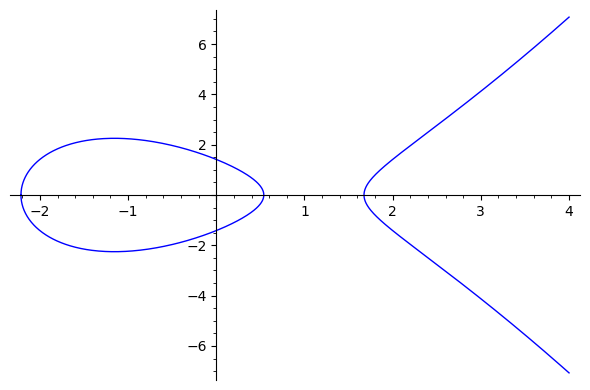
\includegraphics[width=0.8\linewidth]{sage/krzywa_-4_2.png}
    \caption{Krzywa eliptyczna $y^2=x^3-4+2$ nad ciałem liczb rzeczywistych}
    \label{fig:krzywa_rel}
\end{figure}

Krzywe eliptyczne zdefiniowane na liczbach rzeczywistych (rys. \ref{fig:krzywa_rel}) nie są kluczowe w
systemach kryptograficznych \cite*{Stinson2021}, ale takie ustawienia
pozwalają na prostsze przedstawienie niektórych zagadnień
np. dodawanie punktów na krzywej.


\subsubsection{Dodawanie punktów na krzywej eliptycznej}
Odpowiednie zdefiniowanie operacji dodawania punktów na krzywej eliptycznej
pozwala otrzymać grupę abelową, złożoną z punktów krzywej oraz punktu w nieskończoności jako
elementu neutralnego.
\newline
\indent
Geometrycznie, dodawanie punktów na krzywej eliptycznej nad ciałem liczb rzeczywistych można przedstawić
jako połączenie dwóch punktów $P$ i $Q$ prostopadłą linią, która przecina krzywą w trzecim
punkcie, $R'$. Następnie, wynikowy punkt $R$, będący sumą $P+Q$, znajdujemy przez
odbicie punktu $R'$ względem osi $x$ (rys. \ref{fig:krzywa_add}). W przypadku podwojenia punktu, czyli dodawania
punktu P do siebie samego, rysujemy styczną do krzywej w punkcie $P$, która przecina
krzywą w nowym punkcie. Odbicie tego punktu względem osi $x$ daje nam wynik $2P$ \cite{Algorytmy}\cite{Stinson2021}.
\begin{figure}[!h]
    \centering 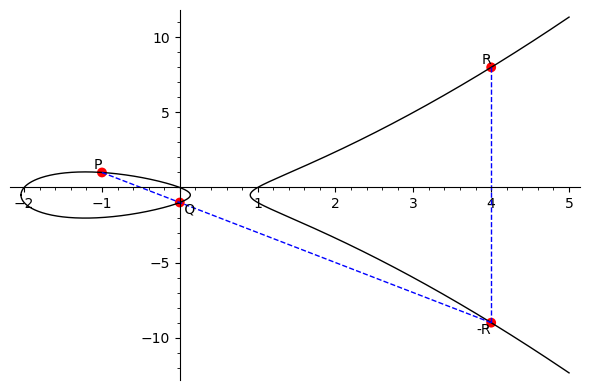
\includegraphics[width=0.8\linewidth]{sage/elliptic_rational_point_addition.png}
    \caption{P + Q na krzywej eliptycznej $y^2+y=x^3-x^2+2x$}
    \label{fig:krzywa_add}
\end{figure}
\par
Definiując dodawanie punktów na krzywej eliptycznej w sposób algebraiczny, otrzymujemy następujące wzory:
\begin{enumerate}
    \item Przypadek, gdy \( P \neq Q \):
          \begin{align}
              \lambda & = \frac{y_2 - y_1}{x_2 - x_1}, \\
              x_3     & = \lambda^2 - x_1 - x_2,       \\
              y_3     & = \lambda(x_1 - x_3) - y_1
          \end{align}
    \item Przypadek, gdy \( P = Q \):
          \begin{align*}
              \lambda & = \frac{3x_1^2 + a}{2y_1}, \\
              x_3     & = \lambda^2 - 2x_1,        \\
              y_3     & = \lambda(x_1 - x_3) - y_1
          \end{align*}
    \item Szczególny przypadek, gdy \( P = -Q \):
          \begin{align*}
              P + (-P) = \mathcal{O}
          \end{align*}
\end{enumerate}
Dodatkowo odwrotność punktu na krzywej $P$ definiujemy jako $-P = (x, -y)$ \cite{Stinson2021}.


\subsubsection{Krzywe eliptyczne na ciele skończonym}
Krzywe eliptyczne zdefiniowane na ciele skończonym $F_p$ oraz $F_{p^n}$ mają kluczowe znaczenie w kryptografii \cite{Stinson2021}.
Praca ta skupia się wyłącznie na krzywych zdefiniowanych na ciele skończonym $F_p$ gdzie $p$ jest liczbą pierwszą.
Wykres krzywej eliptycznej nad ciałem $F_p$ (rys. \ref{fig:krzywa_fp}),
nie przypomina krzywej zdefiniowanej na liczbach rzeczywistych.
Krzywa taka składa się z dyskretnych punktów, których współrzędne należą do ciała
na którym jest opisana.
Operacje na krzywej nad ciałem skończonym są zdefiniowane
za pomocą tych samych wzorów algebraicznych, co w przypadku ciała liczb rzeczywistych,
jednak wszystkie działania są wykonywane na ciele $F_p$.
\begin{figure}[!h]
    \centering 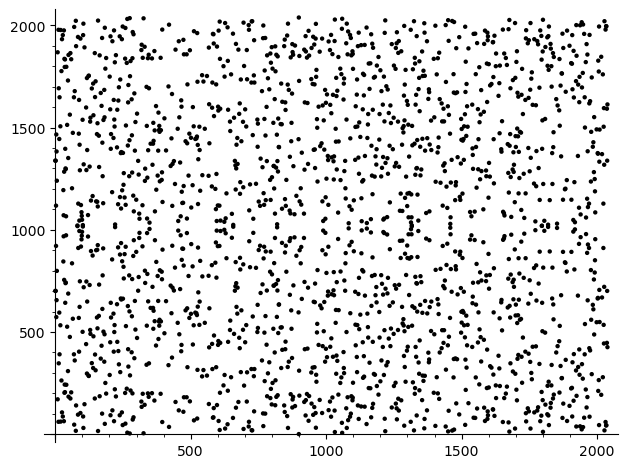
\includegraphics[width=0.8\linewidth]{sage/ec_2_11-9.png}
    \caption{Krzywa eliptyczna $y^2=x^3-4+2$ nad $GF(2^{11} - 9)$}
    \label{fig:krzywa_fp}
\end{figure}


\subsubsection{Problem logarytmu dyskretnego}
Problem logarytmu dyskretnego \textbf{DLP} ( \textit{Discrete Logarithm Problem})
jest podstawą kryptosystemów opartych na grupach.
Jednymi z bardziej znanych są kryptosystem El-Gamala oraz protokół wymiany
kluczy Diffie-Hellmana'a \cite{Stinson2021,Blake2005}.
Problem logarytmu dyskretnego można zdefiniować na grupach cyklicznych,
zarówno na grupie multiplikatywnej $(\mathbb{G},\cdot)$
jak i na grupie addytywnej $(\mathbb{G}, +)$, przy odpowiednim zdefiniowaniu działań grupowych.

Jeżeli G jest multiplikatywną grupą cykliczną a $\gamma$ jej generatorem, to logarytmem dyskretnym
elementu $\alpha \in G$ nazywamy najmniejszą nieujemną liczbę całkowitą $x$ taką, że:
\[x = \log_{\gamma}{\alpha}\]

Uważa się, że problem logarytmu dyskretnego jest trudny obliczeniowo, ponieważ nie istnieje
algorytm, który znajduje $x$ w czasie wielomianowym\cite{Stinson2021}.


\subsubsection{Problem logarytmu dyskretnego na krzywej eliptycznej}
W przypadku kryptografii opartej na krzywych eliptycznych, DLP dotyczy cyklicznej \\
grupy addytywnej $(\mathbb{E},+)$ zdefiniowanej na krzywej eliptycznej.
Aby utworzyć taką grupę, wybieramy punkt $P$ na krzywej eliptycznej $\mathbb{E}$,
który będzie generatorem grupy. Wtedy grupa addytywna $\mathbb{E}$ jest generowana przez
kolejne \textit{potęgi} punktu $P$:
\[\ \langle P \rangle = \{P, 2P, 3P, \ldots, nP = \mathcal{O}\}\]
W takim przypadku, ponieważ operacją na grupie jest dodawanie modulo n, to działanie
potęgowania przedstawia się jako zwielokrotnienie punktu $P$:
\[x \cdot P = Q \textrm{ (mod } n)\]
Analogicznie do problemu logarytmu dyskretnego na grupach multiplikatywnych,
problem logarytmu dyskretnego na krzywej eliptycznej polega na znalezieniu
$x$.
\par
Przy odpowiednim wyborze grupy addytywnej, rozwiązanie problemu logarytmu dyskretnego,
tj. znalezienie $x$,
jest trudne \cite{Stinson2021}.


\subsection{Algorytm Rho Pollard'a}

Zaproponowany przez Johna Pollard'a w 1978 roku \cite{Pollard1978},
algorytm Rho Pollard'a opiera się na wykorzystaniu paradoksu dnia urodzin w celu znalezienia logarytmu dyskretnego.
Pozwala on na znalezienie rozwiązania w czasie $O(\sqrt{n})$,
jednak jest to jedynie czas \textit{oczekiwany}, ze względu na losową naturę algorytmu \cite{Blake2005}.
W porównaniu do innego znanego algorytmu, Baby-Step Giant-Step \cite{Stinson2021}, algorytm Rho Pollard'a jest bardziej
efektywny pamięciowo, nie wymagając
przestrzeni $O(\sqrt{n})$ a jedynie $O(1)$ w wersji sekwencyjnej \cite{Stinson2021}\cite{Blake2005}.
\par

Idea algorytmu polega na losowym błądzeniu po krzywej eliptycznej
w celu znalezienia kolizji dwóch punktów, które spełniają równanie:
$$
    a P + b Q = a' P + b' Q \textrm{ (mod } n)
$$
gdzie $P$ jest generatorem grupy cyklicznej rzędu $n$ na krzywej eliptycznej $\mathbb{E}$ \\
oraz $x \cdot P = Q$, więc $x$ jest szukanym rozwiązaniem problemu.
Gdy znajdziemy kolizję, odpowiednio przekształcając powyższe równanie, możemy znaleźć
$x$:
$$
    x \equiv \frac{(a-a')}{(b'-b)} \textrm{ (mod } n)
$$


Klasyczny algorytm Rho Pollard'a, oparty o poszukiwanie cyklu,
aby znaleźć kolizję, iteracyjne oblicza parę trójek:
$(R_i,a_i,b_i)$ oraz $(R_j,a_j,b_j)$ gdzie $R_j, R_i \in \mathbb{E}$, które spełniają
własność $R = a P + b Q$:
$$
    f(R,a,b) =
    \begin{cases}
        (R + P,a,b+1)     & \text{if } R \in S_1, \\
        (2R,2a, 2b)       & \text{if } R \in S_2, \\
        (R + Q, a + 1, b) & \text{if } R \in S_3,
    \end{cases}
$$
natomiast $S_1 \cup S_2 \cup S_3$ jest podziałem $\mathbb{E}$ na trzy podzbiory, które powinny być podobnej wielkości.
Ponieważ $R$ jest punktem na krzywej eliptycznej a nie liczbą całkowitą, często stosowanym sposobem
podziału różnych wartości $R$ na trzy zbiory, jest obliczanie operacji modulo $3$ ze współrzędnej $x$.
Aby z kolejno obliczanych trójek znaleźć kolizję punktów, zazwyczaj stosuje się algorytm poszukiwania cyklu Floyd'a.
W takim przypadku, w każdej iteracji oblicza się trójki: $(R_i, a_i, b_i)$ oraz $(R_{2i}, a_{2i}, b_{2i})$, aż do znalezienia
kolizji $R_i = R_{2i}$.

\par
Sekwencyjna wersja algorytmu słabo się skaluje w przypadku zwiększania ilości równolegle działających procesorów,
osiągając jedynie przyśpieszenie rzędu $O(\sqrt{m})$ dla $m$ procesorów \cite{Oorschot}.
Dlatego w swojej pracy wykorzystałem równoległą wersję algorytmu, zaproponowaną przez Van Oorschota i Wienera \cite{Oorschot}.

\subsubsection{Równoległy algorytm Rho Pollard'a}
Równoległa wersja algorytmu Rho Pollard'a, zakłada zastosowanie wielu równolegle działających
procesorów, które niezależnie od siebie wykonują \textit{spacer losowy} po krzywej eliptycznej,
w poszukiwaniu \textit{punktów wyróżnionych}. Gdy znajdą taki punkt, przekazują go do serwera centralnego,
który odpowiada za gromadzenie znalezionych punktów wyróżnionych oraz poszukiwanie kolizji między nimi.
\par
Cecha określająca czy dany punkt na krzywej jest wyróżniony, powinna być łatwo weryfikowalna i tania obliczeniowo,
ponieważ sprawdzenie czy dany punkt jest wyróżniony, występuje w każdej iteracji algorytmu.
\par
Często wybieranym sposobem sprawdzenia czy punkt jest wyróżniony, jest obliczenie ilości zer na początku lub na końcu
reprezentacji bitowej jednej ze współrzędnych punktu. Różny dobór tej cechy wpływa na pamięć oraz
czas wymagany do znalezienia kolizji. Bardzo szeroki zakres punktów które spełniają kryteria bycia wyróżnionymi,
spowoduje bardzo szybkie zapełnienie pamięci centralnego serwera a za wąski spowoduje, że czas do znalezienie kolizji się wydłuży.

\subsubsection{Adding Walk}
Adding Walk jest modyfikacją funkcji iteracyjnej $f$ używanej w algorytmie Rho Pollard’a
do obliczania kolejnych punktów na krzywej eliptycznej \cite{Teske2000}. Funkcja ta opiera się 
na dodawaniu w każdej iteracji punktów z predefiniowanej tablicy punktów, co 
zapewnia wysoką efektywność oraz równomierny rozkład iteracji w grupie. Wprowadzenie 
Adding Walk, jak pokazano w pracy Teske \cite{Teske2000}, poprawia wydajność w 
stosunku do oryginalnej wersji algorytmu, zapewniając prostszą implementację w 
przypadku równoległych obliczeń, takich jak te wykonywane na GPU.

Niech $W_0 = nP$ będzie punktem startowym, gdzie $n$ to znana wielokrotność 
generatora grupy $P$. Funkcja iteracyjna $f$ jest zdefiniowana jako odwzorowanie 
$f: \langle P \rangle \rightarrow \{1, \ldots, s\}$ o możliwie równomiernym 
rozkładzie. Następnie należy zdefiniować tablicę predefiniowanych punktów:
$$
R_i = c_i P + d_i Q, \quad \text{dla } 0 \leq i \leq s - 1,
$$
gdzie $c_i$ i $d_i$ są współczynnikami losowymi. Funkcja iteracyjna jest zdefiniowana 
jako:
$$
W_{i+1} = W_i + R_{f(W_i)}.
$$
Podczas każdej iteracji konieczne jest zliczanie współczynników odpowiadających 
wielokrotnościom $P$ i $Q$, aby każdy punkt na krzywej mógł zostać jednoznacznie 
przedstawiony w postaci $aP + bQ$. Suma współczynników $a$ i $b$ jest aktualizowana 
w każdej iteracji zgodnie z wartościami predefiniowanych współczynników 
$c_i$ i $d_i$ dla punktu $R_{f(W_i)}$. Zliczanie tych wartości jest kluczowe 
dla odtworzenia obliczeń w przypadku znalezienia kolizji, umożliwiając późniejsze 
wyznaczenie logarytmu dyskretnego.

Istotnym czynnikiem jest również rozmiar tablicy $s$, który ma spore znaczenie
dla skuteczności algorytmu. Zbyt mała 
wartość $s$ może powodować, że funkcja iteracyjna nie będzie wystarczająco 
"losowa". Eksperymenty wykazały, że dla $s \geq 16$, funkcja $f$ zapewnia 
odpowiedni poziom losowości, niezależnie od rozmiaru grupy \cite{Teske2000}.

Główną zaletą tej metody w implementacjach GPU jest minimalizacja rozgałęzień 
w czasie iteracji. Dzięki temu niemal wszystkie wątki wykonują tę samą operację 
dodawania punktów, co jest istotne w architekturze SIMD. Wyjątkiem jest rzadki przypadek, gdy $W_i = R_{f(W_i)}$, co 
wymaga wykonania operacji zwielokrotnienia punktu.

\newpage
\section{Koncepcja}

Projekt systemu do obliczania logarytmu dyskretnego wykorzystuje koprocesor GPU w celu akceleracji obliczeń.
Równoległy algorytm Rho Pollard'a opiera się na architekturze, w której centralny serwer zbiera wyniki
z wielu jednostek obliczeniowych. W związku z tym system składa się z dwóch głównych elementów:
programu pełniącego rolę centralnego serwera oraz programu klienta, wykonującego obliczenia na GPU,
który może być uruchamiany w wielu instancjach.
Oba programy, zarówno serwer, jak i klient, mogą działać na jednym komputerze
lub w środowisku maszyny wirtualnej, komunikując się za pomocą mechanizmów IPC.
Architektura została zaprojektowana w sposób umożliwiający wykorzystanie wielu kart graficznych
podłączonych do komputera, co dodatkowo zwiększa wydajność obliczeń.

\subsection{Klient}
Klient składa się z dwóch wyróżnionych części.
Część odpowiedzialna za obliczenia na krzywej została napisana w języku
CUDA C++. W celu optymalizacji obliczeń pod platformę GPU, algorytm oblicza
kolejne punkty za pomocą \textit{Adding Walk}, opisanego w poprzednim
rozdziale. W tym celu niezbędne jest zaimplementowanie operacji modularnych,
które umożliwiają przeprowadzanie obliczeń na krzywej eliptycznej.

Ponieważ w języku C oraz CUDA C++ nie istnieje typ danych pozwalający na
przechowywanie liczb większych niż 64-bitowe, konieczne jest odpowiednie
zaimplementowanie nowych typów danych oraz samych operacji na \textit{długich liczbach}.

Aby rozpocząć obliczenia, program klienta otrzymuje następujące dane wejściowe:
\begin{itemize}
    \item tablicę punktów startowych,
    \item ziarna użyte do wygenerowania każdego z punktów startowych,
    \item tablicę punktów wstępnie obliczonych potrzebnych do \textit{Adding Walk},
    \item parametry krzywej.  
\end{itemize}
Ziarno używane do generowania punktów startowych jest w postaci liczby, przez
którą należy zwielokrotnić punkt $P$, aby otrzymać dany punkt startowy.
Po otrzymaniu danych, program uruchamia kernel CUDA, odpowiedzialny za szukanie punktów wyróżnionych.
Każdy uruchomiony wątek, niezależnie od pozostałych, przeprowadza obliczenia algorytmu, aż do momentu
gdy znajdzie punkt wyróżniony.
Jako wynik działania, program zwraca
tablicę punktów wyróżnionych, wraz z odpowiadającymi im ziarnami punktów startowych, od których zaczeły
się obliczenia prowadzące do danego wyniku. \\
Druga część programu klienta, jest napisana w języku Python i stanowi wysokopoziomowy interfejs do komunikacji
z serwerem. W jej skład wchodzi moduł odpowiedzialny za wywoływanie skompilowanej części kodu za pomocą ABI języka C,
oraz kod funkcji, która jest uruchamiana jako oddzielny wątek z poziomu programu serwera. W celu komunikacji
między wątkami wykorzystywana jest implementacja kolejki asynchronicznej z biblioteki standardowej.
Po uruchomieniu nowego wątku, na początku działania otrzymuje on parametry krzywej i pracuje
on aż do znalezienia rozwiązania ECDLP i zakończenia wszystkich wątków przez serwer.
W trakcie pracy, wątek klienta przyjmuje kolejne punkty startowe przesłane przez serwer za pomocą kolejki
oraz zwraca obliczone punkty wyróżnione wraz z ziarnami.

\subsection{Serwer}
Serwer, w całości zaimplementowany w języku Python, pełni kluczową rolę w systemie,
zajmując się gromadzeniem punktów wyróżnionych przesyłanych przez działające wątki klientów oraz wyszukiwaniem
kolizji pomiędzy nimi. Jego zadania obejmują również zarządzanie pracą
wątków klientów, polegające na dynamicznym uruchamianiu odpowiedniej liczby instancji
oraz zapewnianiu mechanizmów komunikacji za pomocą kolejek.
Do efektywnego przechowywania punktów wyróżnionych zastosowano strukturę danych w formie
hash mapy, w której kluczami są współrzędne punktów.
Rozwiązanie to umożliwia szybkie wyszukiwanie potencjalnych kolizji,
co znacząco zwiększa wydajność procesu.
Serwer również musi być zdolny do odtworzenia pełnego przebiegu obliczeń dowolnego klienta w przypadku,
gdy jeden z jego punktów wyróżnionych stanie się elementem kolizji.
Aby to osiągnąć, serwer implementuje tę samą logikę obliczeniową co klient,
co zapewnia spójność wyników. Dzięki temu, na podstawie ziarna punktu startowego, serwer zawsze uzyskuje identyczne
rezultaty jak klient.
W przeciwieństwie do klienta,
serwer dodatkowo śledzi sumę wielokrotności punktów $P$ i $Q$,
co jest niezbędne do późniejszego obliczenia logarytmu dyskretnego.

\subsection{Przepływ działania}
W momencie uruchomienia programu, serwer generuje wyznaczoną liczbę punktów wstępnie obliczonych.
Punkty te będą przechowywane przez serwer aż do końca działania programu, wraz z parametrami, które
wygenerowały każdy z tych punktów. Następnie serwer uruchamia w wielu wątkach funkcję napisaną w pythonie, która
odpowiada za nadzorowanie pracy programu klienta GPU. Każda z uruchomionych funkcji w momencie startu
otrzymuje adres dwóch kolejek, które będą służyły do komunikacji z głównym wątkiem serwera. \\
Po uruchomieniu wątków, serwer rozpoczyna działanie pętli, która zakończy się dopiero po znalezieniu
rozwiązania ECDLP. W trakcie jej działania, serwer wykonuje następujące kroki:
\begin{enumerate}
    \item Generacja nowych punktów startowych
    \item Przekazanie punktów startowych do kolejki zadań
    \item Pobranie znalezionych punktów wyróżnionych z kolejki z wynikami
    \item Sprawdzenie czy w bazie punktów znalezionych wystąpiła kolizja
    \item Dodanie punktów do bazy punktów znalezionych
\end{enumerate}
W momencie gdy serwer znajdzie kolizję dwóch punktów, podejmuje on próbę znalezienia ECDLP.
Jeżeli wynik został poprawnie obliczony, serwer kończy działanie całego programu, wraz z wątkami klientów.
\par
Podprogramy klientów, uruchomione w osobnych wątkach,
również działają w pętli, w trakcie której wykonują następujące kroki:
\begin{enumerate}
    \item Odebranie punktów startowych z kolejki zadań
    \item Uruchomienie obliczeń na GPU
    \item Odebranie wyników z GPU
    \item Przekazanie znalezionych punktów wyróżnionych do kolejki z wynikami
\end{enumerate}
Komunikacja z programem na GPU odbywa się za pomocą \textit{Ctypes}, przekazując
do programu GPU tablice z języka C oraz strukturę z danymi o parametrach krzywej,
na której prowadzone są obliczenia.
\begin{figure}[!h]
    \centering 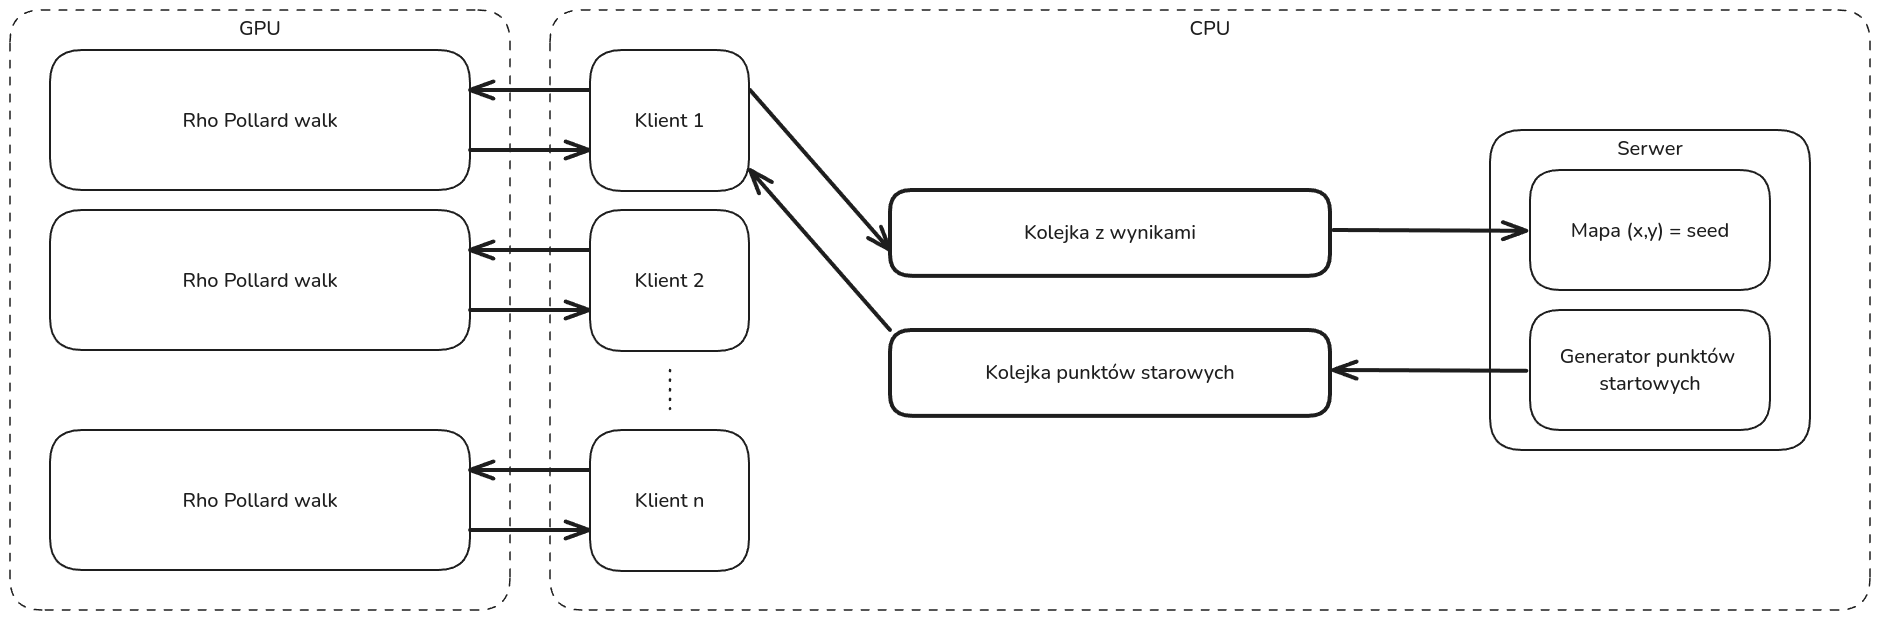
\includegraphics[width=1.1\linewidth]{arch.png}
    \caption{Schemat architektury}
\end{figure}

\newpage
\section{Implementacja}
Ta część pracy jest poświęcona implementacji całego systemu,
wraz ze szczegółowym opisem narzędzi oraz sprzętu wykorzystanego
przy pracy nad projektem.
\par
Większość opisanych zagadnień dotyczy części klienta napisanej w CUDA C++,
poza sekcją na końcu, poświęconą serwerowi oraz części klienta działającej na CPU.

\subsection{Narzędzia oraz sprzęt}
\subsubsection{Sprzęt}
\begin{itemize}
    \item OS: openSUSE Tumbleweed 20240812
    \item CPU: Intel Core i5-10600KF 4.10 GHz
    \item RAM: 16 GB
    \item GPU: GeForce RTX 2070 Super
\end{itemize}

\subsubsection{Program po stronie CPU}
Implementacja programu serwera działającego po stronie CPU, została wykonana z wykorzystaniem
języka Python w wersji 3.11.1 wraz z pakietem obliczeniowym SageMath w wersji 10.4.beta3.
Program klienta został zaimplementowany z wykorzystaniem języka Python w wersji 3.11.1 oraz
języka CUDA C++ w wersji 12.4.

\subsubsection{System budowania oraz kompilacja CUDA C++}
W celu zarządzania kompilacją części projektu napisanej w języku CUDA oraz C++,
wykorzystałem narzędzie \textit{CMake}.
\textit{CMake} zapewnia natywne wsparcie dla języka CUDA,
co znacznie upraszcza wszelkie zarządzanie kompilacją oraz linkowanie.
Dodatkowo, wymaga to znacznie mniej wstępnej konfiguracji niż analogiczne
rozwiązanie z wykorzystaniem samego narzędzia do budowania takiego jak \textit{Make} lub \textit{Ninja}.
\par
Program napisany w CUDA kompilowany był z wykorzystaniem kompilatora NVCC dostarczonego wraz z pakietem
\textit{CUDA Toolkit} w wersji 12.4.
NVCC do kompilacji kodu po stronie host'a (CPU) wykorzystuje kompilator z GCC w wersji 13.3.1.


\subsubsection{Testy}
Wszelkie testy poprawności implementacji rozwiązania są przeprowadzane z wykorzystaniem framework'a PyTest dla języka Python.
Python wraz z wykorzystaniem pakietu obliczeniowego SageMath generuje testowe dane, które
są przekazywane do programu działającego na GPU. Następnie, otrzymane wyniki są porównywane z rezultatami
obliczonymi przy wykorzystaniu SageMath. Wykorzystanie PyTest oraz SageMath znacznie przyśpieszyło pracę
nad implementacją operacji na krzywej eliptycznej oraz docelowej implementacji algorytmu Rho Pollard'a.
Możliwość szybkiego generowania dużych zbiorów danych testowych, pozwoliło na wczesne zauważenie wielu subtelnych błędów
na etapie implementacji.


\subsection{Program klienta Python}
Część podprogramu klienta napisana w języku Python, została zaimplementowana
za pomocą biblioteki \textit{Threading} z biblioteki standardowej.
Na początku działania programu, podprogram serwera uruchamia w kilku wątkach
funkcję \textit{GPUWorker} która stanowi implementację klienta.
Odpowiada ona za
dostosowywanie danych wejściowych do programu napisanego w CUDA, oraz
zwracanie wyników z powrotem do serwera. Sygnatura funkcji GPUWorker:
\begin{lstlisting}[language=Python]
def GPUworker(
    starting_params: StartingParameters,
    task_queue: Queue,
    result_queue: Queue, stream):
\end{lstlisting}

W celu komunikacji z serwerem, wykorzystywane są obiekty kolejek
\textit{queue.Queue} z biblioteki standardowej.
Ponieważ Python w wersji 3.12 nie wspiera równoległego wykonywania
się wątków, to zmiana wątku następuje po wywołaniu programu CUDA.
Następuje wtedy wywołanie systemowe \textit{Sleep} i wątek pozostaje nieaktywny
aż do zakończenie obliczeń przez GPU.
Dzięki kompilacji programu CUDA z flagą \textit{--default-stream per-thread},
każdy z wątków klienta uruchamia program na GPU w innym strumieniu CUDA. Pozwala
to na współbieżne wykonywanie się obliczeń na GPU uruchomionych przez każdy wątek, zarządzane przez
\textit{CUDA Scheduler}. \\
Implementacja struktur danych przekazywanych do programu CUDA:
\begin{lstlisting}[language=Python]
LIMBS = 5
class bn(ctypes.Structure):
    _fields_ = [("array", ctypes.c_uint32 * LIMBS)]

class small_bn(ctypes.Structure):
    _fields_ = [("array", ctypes.c_uint32 * ceil(LIMBS / 2))]
class EC_point(ctypes.Structure):
    _fields_ = [
        ("x", bn),
        ("y", bn),
        ("seed", bn),
        ("is_distinguish", ctypes.c_uint32),
    ]
\end{lstlisting}

\subsection{Program klienta CUDA}

Program uruchamiany na GPU został skompilowany jako dynamicznie linkowana
biblioteka (\textit{SHARED}). Aby zapewnić zgodność z interfejsem binarnym
(ABI) wykorzystywanym przez bibliotekę Ctypes, do głównej funkcji dodano
słowo kluczowe \texttt{extern "C"}.
Pozwoliło to uzyskać punkt wejścia zgodny
z konwencją wywołania C (C ABI). Główna funkcja, po otrzymaniu parametrów
startowych, alokuje odpowiednią pamięć CUDA oraz konfiguruje niezbędne
parametry uruchamiana dla głównego kernel'a, który realizuje algorytm
Rho Pollard'a. Po zakończeniu obliczeń, pamięć jest zwalniana, a wyniki
zapisywane w tablicach przekazanych jako dane wejściowe. W rezultacie,
tablica punktów startowych przekazana do programu pełni jednocześnie
funkcję miejsca zapisu wyników obliczeń.
Prototyp funkcji wejściowej do programu CUDA:
\begin{lstlisting}[language=C++]
extern "C" {
void run_rho_pollard(
    EC_point *startingPts,
    uint32_t instances,
    uint32_t n, PCMP_point *precomputed_points,
    EC_parameters *parameters,
    int stream
    )
\end{lstlisting}
Następne podrozdziały są poświęcone implementacji poszczególnych
elementów składających się na kod głównego kernel'a CUDA.


\subsection{Arytmetyka na ciele}
\subsubsection{Reprezentacja długich liczb}
W przypadku ciała $F_{p}$, gdzie $p$ jest liczbą pierwszą o rozmiarze 79 bit, potrzebujemy co najmniej 79 bitowego typu danych, do samego przechowywania liczb.
Jednak nawet 79 bitowy typ danych nie wystarczy, jeżeli chcemy przeprowadzić operację mnożenia
dwóch liczb 79 bitowych. W takim przypadku, wynik pośredni może być maksymalnie $2*79 = 158$ bitowy.
Dodatkowo, w celu reprezentacji takiej liczby, nie możemy się posłużyć wektorem składającym się z największego
dostępnego natywnie typu danych,
ponieważ wyniki pośrednie z operacji mnożenia lub dodawania mogą przekroczyć rozmiar słowa bitowego.
W tym celu musimy wykorzystać typ danych mniejszy od maksymalnego. W przypadku CUDA C++, największy wspierany typ danych
wynosi 64 bit, więc w celu reprezentacji liczb, musiałem wykorzystać wektor składający się z 32 bitowych słów.
Najbliższa wielokrotność liczby 32 bitowej, większa niż 158 bit to 160 bit,
dlatego w celu reprezentacji liczb na ciele, wykorzystywany jest wektor postaci:
$$
    \sum_{i = 0}^{4} x_i\cdot 2^{32}
$$

Zaimplementowany jako tablica typu u\_int32:
\begin{lstlisting}[language=C++]
struct bn
{
    uint32_t array[5];
};
\end{lstlisting}
Dla liczb, na których bezpośrednio nie będą wykonywane operacje arytmetyczne, wykorzystywany jest mniejszy, tymczasowy typ
danych.
Ograniczone zasoby szybkiej pamięci współdzielonej na GPU, wymuszają oszczędne zarządzanie pamięcią. W celu
przechowywania wstępnie obliczonych punktów w pamięci współdzielonej, wykorzystuję następujący typ danych:
\begin{lstlisting}[language=C++]
struct small_bn
{
    uint32_t array[3];
};
\end{lstlisting}
\par
Liczby w takiej postaci, przed przeprowadzeniem na nich operacji arytmetycznych, są ładowane z pamięci współdzielonej i z powrotem konwertowane na większy typ danych.
Pozwala to zaoszczędzić $ 2 \cdot 32$ bitów na każdej liczbie, co w przypadku punktu składającego się z dwóch współrzędnych
daje oszczędność $2 \cdot 2 \cdot 32 = 128$ bitów na punkt znajdujący się w pamięci.

\subsubsection{Operacje na długich liczbach}
Do operacji na długich liczbach, odpowiednio dostosowałem małą bibliotekę
dostępną w domenie publicznej: \textit{tiny-bignum-c}.
Biblioteka ta dostarcza podstawowe operacje na dużych liczbach w postaci wektorów, takie jak dodawanie, odejmowanie, mnożenie czy dzielenie.
Wykorzystuje w tym celu standardowe algorytmy \cite{Menezes2001} wykorzystywane przy obliczeniach \textit{multiple precision}.
Dużą zaletą ten biblioteki jest jej prostota i brak wykorzystania standardowej biblioteki C oraz dynamicznej alokacji pamięci.
Wszystkie operacja są wykonywane z wykorzystaniem stosu,
co pozwala na jej wykorzystanie w środowiskach takich jak GPU, gdzie dostęp do dynamicznej alokacji pamieci jest ograniczony.
W większości przypadków, aby dostosować kod z biblioteki do CUDA C++ wystarczyło dodanie
odpowiedniej dyrektywy \textit{\_\_device\_\_} przed każdą deklaracją funkcji, która informuje kompilator, że dana funkcja
będzie wykonywana na GPU.
\par
Prymitywy matematyczne dostarczane przez bibliotekę \textit{tiny-bignum-c} nie są jednak wystarczające do przeprowadzenia
operacji na ciele $F_{p}$.
W związku z tym, zaimplementowałem dodatkowe operacje modularne takie jak mnożenie, dodawanie, odejmowanie i odwrotność modulo.

\subsubsection{Dodawanie i odejmowanie modulo}
Dodawanie oraz odejmowanie modulo $p$, wygląda bardzo podobnie do standardowego dodawania i odejmowania.
\par
W przypadku odejmowanie dwóch liczb na ciele $F_{p}$, nie ma potrzeby redukcji modulo p po każdej operacji.
Jednak niezbędne jest upewnienie się, że wynik nie jest ujemny. Ponieważ prowadzimy obliczenia na liczbach bez znaku,
to w sytuacji gdy $a - b = c; a < b$, nastąpi przepełnienie i wynik będzie w postaci $2^{32 \cdot n}-1 - c$, gdzie $n$ to rozmiar
wektora do przechowywania liczb. Na szczęście, możemy bardzo łatwo wrócić do poprawnego wyniku wykorzystując jedną operację
dodawania. Korzystając z faktu, że wszystkie podstawowe operacje są wykonywane modulo $2^{32 \cdot n}$:
$$
    2^{32 \cdot n} - 1 - c + p \equiv p - c \pmod{2^{32 \cdot n}}
$$
Przykładowa implementacja z wykorzystaniem \textit{tiny-bignum-c}:

\begin{lstlisting}[language=C++]
bignum_sub(a, b, c);
if (bignum_cmp(a, b) == SMALLER)
{
    bignum_add(c, p, temp);
    bignum_assign(c, temp);
}
\end{lstlisting}
\par
Dodawanie modulo $p$ jest prostsze.
Aby wykonać dodawanie modularne, wystarczy wykonać standardowe dodawanie i ewentualnie jeżeli $a + b >= p$ zredukować wynik odejmując
od niego liczbę p.

\subsubsection{Mnożenie modulo}
Mnożenie modularne jest bardziej kosztowne niż dodawanie czy odejmowanie, ponieważ wymaga dzielenia z resztą.
W swojej pracy przeprowadzam standardowe mnożenie modularne, jednak również istnieją bardziej wydajne sposoby, na przykład wykorzystanie redukcji Barret'a CITE APPLIED.
\par
Aby przeprowadzić klasyczne mnożenie modularne ciele $F_{p}$, na początku musimy przeprowadzić standardowe mnożenie długich liczb.
Następnie, otrzymany wynik dzielimy przez $p$ i zwracamy resztę z dzielenia.
Zarówno mnożenie jak i dzielenie z resztą, są funkcjami dostarczonymi
w bibliotece \textit{tiny-bignum-c}, więc mnożenie modularne sprowadza się do wykonania tych dwóch operacji jedna po drugiej.

\subsubsection{Odwrotność modulo}
Obliczanie odwrotności modulo $p$ jest najbardziej kosztowną operacją na ciele $F_{p}$, głównie ze względu
na wielokrotne dzielenie w pętli.
Algorytm obliczania odwrotności modulo $p$ zaimplementowałem z wykorzystaniem rozszerzonego algorytmu Euklidesa,
który został zmodyfikowany do działania na liczbach nieujemnych. Główna różnica względem klasycznego algorytmu,
polega na wykorzystaniu dodatkowych zmiennych do śledzenia zmian znaku wyniku.

\begin{algorithm}[]
    \caption{Odwrotność modularna a mod b}
    \label{alg:inverse}
    \begin{algorithmic}[1]
        \State \text{\textbf{Input: }} $a, b$
        \State $b_0 \gets b$
        \State $x_0 \gets 0$
        \State $x_1 \gets 1$
        \State $x_{0\_sign} \gets 0$
        \State $x_{1\_sign} \gets 0$

        \While{$a > 1$}
        \State $q \gets a \div b$
        \State $t \gets b$
        \State $b \gets a \mod b$
        \State $a \gets t$

        \State $t_2 \gets x_0$
        \State $t_{2\_sign} \gets x_{0\_sign}$
        \State $qx_0 \gets q \times x_0$

        \If{$x_{0\_sign} \neq x_{1\_sign}$}
        \State $x_0 \gets x_1 + qx_0$
        \State $x_{0\_sign} \gets x_{1\_sign}$
        \Else
        \If{$x_1 > qx_0$}
        \State $x_0 \gets x_1 - qx_0$
        \State $x_{0\_sign} \gets x_{1\_sign}$
        \Else
        \State $x_0 \gets qx_0 - x_1$
        \State $x_{0\_sign} \gets 1 - x_{0\_sign}$
        \EndIf
        \EndIf

        \State $x_1 \gets t_2$
        \State $x_{1\_sign} \gets t_{2\_sign}$
        \EndWhile
        \If{$x_{1\_sign} == 1$}
        \State \Return $b - x_1$
        \Else
        \State \Return $x_1$
        \EndIf

    \end{algorithmic}
\end{algorithm}


\subsubsection{Biblioteka CGBN}
W pierwotnej wersji swojej pracy, do operacji na dużych liczbach wykorzystałem specjalną bibliotekę CGBN dla platformy CUDA. Oferuje ona
wszystkie podstawowe operacje na długich liczbach, takie jak dodawanie, odejmowanie czy mnożenie nawet do 32 tyś. bitów.
Dodatkowo, posiada ona implementację bardziej zaawansowanych funkcji, takich jak odwrotność modulo czy redukcja Barret'a.
Niestety, biblioteka ta narzuca spore ograniczenia pod kątem zasobów. Niezbędne jest grupowanie wątków w grupy
4, 8, 16 lub 32. Wysoką wydajność obliczeń, uzyskiwałem dopiero w grupach składających się z 32 wątków.
Pomimo znacznie szybszego wykonywania się poszczególnych operacji w ramach takiej grupy wątków, narzucone
ograniczenia oraz wysokie użycie rejestrów uniemożliwiało
efektywne zaimplementowanie dużej ilości takich instancji działających równolegle.
Całkowita wydajność mierzona w ilości operacji na krzywej na sekundę osiągnięta z jej wykorzystaniem była średnio 4.57 razy gorsza, niż
z wykorzystaniem znacznie prostszej implementacji na bazie \textit{tiny-bignum-c}.

\begin{lstlisting}[language=C, caption=Prototypy funkcji wykorzystywanych do operacji na długich liczbach]
__device__ void bignum_init(struct bn *n);
__device__ void bignum_from_int(struct bn *n, DTYPE_TMP i);
__device__ int bignum_to_int(struct bn *n);

__device__ void bignum_add(struct bn *a, struct bn *b, struct bn *c);
__device__ void bignum_sub(struct bn *a, struct bn *b, struct bn *c);
__device__ void bignum_mul(struct bn *a, struct bn *b, struct bn *c);
__device__ void bignum_div(struct bn *a, struct bn *b, struct bn *c);
__device__ void bignum_mod(struct bn *a, struct bn *b, struct bn *c);
__device__ void bignum_divmod(
    struct bn *a, struct bn *b, struct bn *c, struct bn *d
);

__device__ void bignum_assign_fsmall(struct bn *dst, struct small_bn *src);
__device__ void bignum_assign_small(struct small_bn *dst, struct small_bn *src);

__device__ void bignum_modinv(struct bn *a, struct bn *b, struct bn *c);

__device__ void bignum_and(struct bn *a, struct bn *b, struct bn *c);
__device__ void bignum_or(struct bn *a, struct bn *b, struct bn *c);
__device__ void bignum_xor(struct bn *a, struct bn *b, struct bn *c);
__device__ void bignum_lshift(struct bn *a, struct bn *b, int nbits);
__device__ void bignum_rshift(struct bn *a, struct bn *b, int nbits);

__device__ int bignum_cmp(struct bn *a, struct bn *b);
__device__ int bignum_is_zero(struct bn *n);
__device__ void bignum_inc(struct bn *n);
__device__ void bignum_dec(struct bn *n);
__device__ void bignum_assign(struct bn *dst, struct bn *src);
\end{lstlisting}

\subsection{Funkcja iterująca}

Główna funkcja realizująca kolejne kroki algorytmu Rho Pollard'a została
zaimplementowana jako kernel GPU. Na początku swojego działania kernel ładuje
punkty wstępnie obliczone do pamięci współdzielonej (\textit{shared memory}),
która pełni funkcję pamięci podręcznej.

Pierwszy wątek każdego bloku inicjalizuje specjalną flagę \texttt{warp\_finished},
ustawiając jej wartość na \texttt{0}. Flaga ta służy do kontrolowania zakończenia
pracy wszystkich wątków w ramach danego bloku. Po zakończeniu obliczeń przez
przynajmniej jeden wątek, flaga sygnalizuje konieczność zakończenia działania
pozostałych wątków w bloku. Szczegółowe omówienie mechanizmu działania tej flagi
znajduje się w sekcji poświęconej (\textit{tail effect}).

Przykładowy fragment kodu ilustrujący inicjalizację pamięci współdzielonej oraz
obsługę flagi:

\begin{lstlisting}[language=C, caption=Inicjalizacja pamięci współdzielonej i flagi \texttt{warp\_finished}]
if (threadIdx.x == 0)
{
    printf("STREAM %d BLOCK %d started\n", stream, blockIdx.x);
    for (int i = 0; i < PRECOMPUTED_POINTS; i++)
    {
        bignum_assign_small(&SMEMprecomputed[i].x, &args.precomputed[i].x);
        bignum_assign_small(&SMEMprecomputed[i].y, &args.precomputed[i].y);
    }
    warp_finished = 0;
}
__syncthreads();
\end{lstlisting}

\subsubsection{Wstępnie obliczone punkty}
Dostęp do wstępnie obliczonych punktów jest niezbędny w każdej iteracji \textit{Addition walk}.,
dlatego ważne jest, aby je przechowywać w szybkiej pamięci. Wykorzystałem w tym celu pamięć współdzieloną \textit{shared memory}.
W przeciwieństwie do znacznie większej pamięci globalnej, jest ona przechowywana bezpośrednio na SM \cite{Cheng2014,Jason2011}.
Ponieważ ilość punktów która zapewnia dostatecznie losowy spacer po krzywej eliptycznej
jest stosunkowo niewielka \cite{Teske2000},
to rozmiar pamięci nie stanowi problemu. W docelowej wersji, przechowywane jest 128 punktów.
\par
Funkcja przydzielająca punkt wstępnie obliczony, na podstawie aktualnie sumowanego punktu została zaimplementowana
poprzez operację AND maski bitowej z pierwszymi 64 bitami współrzędnej
$x$ punktu.
W ten sposób, każdy punkt $W_i$ jest przyporządkowany do jednego z 128 wstępnie obliczonych punktów,
a następnie punkty są dodawane do siebie.

\begin{lstlisting}[language=C, caption=Funkcja przydzielająca punkt]
#define PRECOMPUTED_POINTS 128
__device__ uint32_t map_to_index(bn *x) {
    return (x->array[0] & (PRECOMPUTED_POINTS - 1));
}
\end{lstlisting}


\subsubsection{Punkty wyróżnione}
W ramach każdej iteracji, musimy w wydajny i szybki sposób sprawdzić, czy obliczony punkt jest punktem wyróżnionym.
W mojej implementacji, kryterium warunkującym jest liczba zer na końcu współrzędnej $x$ obliczonego punktu.
\par
Do sprawdzenia, czy punkt jest wyróżniony, słuzy prosta funkcja obliczająca bitową operację AND ze
współrzędnej punktu oraz specjalnej maski bitowej wyznaczanej na podstawie poszukiwanej ilości zer.
Przykładowo, dla poszukiwanej liczby zer 3, maska będzie w postaci $0 ... 00111$. Jeżeli
również ostatnie 3 bity współrzędnej $x$ będzie miało zerowy znak, to otrzymany wynik operacji AND wyniesie 0.
\par
Istotne jest, aby taka sama funkcja została zaimplementowana po stronie serwera na CPU, ponieważ w przypadku znalezienia kolizji,
musi on być w stanie odtworzyć cały spacer losowy prowadzący do danego punktu wyróżnionego.

\begin{algorithm}
    \caption{Funkcja \texttt{is\_distinguish}}
    \begin{algorithmic}[1]
        \State \textbf{Input:} $x$, $liczba\_zer$
        \State $mask \gets 1 \ll liczba\_zer - 1$

        \If{$(x \ \& \ mask) == 0$}
        \State \Return \textbf{true}
        \Else
        \State \Return \textbf{false}
        \EndIf
    \end{algorithmic}
\end{algorithm}

\par
Aby ułatwić testy na różnych etapach implementacji całego systemu,
liczba sprawdzanej ilości zer jest sparametryzowana. Przy starcie każdej serii obliczeń, poszukiwana liczba zer jest jednym z parametrów przekazywanym
do funkcji kernel'a.
\par
Po znalezieniu punktu wyróżnionego, ustawiana jest specjalna flaga w strukturze przechowującej dane punktu oraz
jest on zapisywany pod pierwsze wolne miejsce w pamięci globalnej.

\subsubsection{Obliczanie odwrotnosci w seriach}
Każda operacja dodawania punktów na krzywej eliptycznej we współrzędnych afinicznych, składa się z 3 mnożeń modularnych oraz jednej operacji obliczania odwrotności w ciele.
Przeprowadza się również operację dodawania i odejmowania modularnego, jednak ich koszt obliczeniowy jest pomijalnie mały \cite{Blake2005}.
\par
Koszt dodawania punktów na krzywej:
$$
    1O + 3M
$$
Najdroższym działaniem, które wpływa na wysoki koszt obliczeniowy  mnożenia modularnego oraz odwrotności w ciele,
jest operacja dzielenia \cite{Menezes2001}.
Przykładowo, wykorzystywana przeze mnie implementacja dzielenia stosuje prosty algorytm \textit{long division},
o złożoności obliczeniowej $O(n^2)$.
\par
Warto zauważyć, że operacja obliczania odwrotności modularnej z wykorzystaniem algorytmu euklidesa, wykonuje dzielenie
podczas obliczania modulo, na każdym etapie pętli wewnątrz algorytmu \ref{alg:inverse}.
To czyni ją najdroższą operacją na ciele, znacznie kosztowniejszą niż operacja mnożenia modularnego.
\par
Aby przyśpieszyć obliczenia, zastosowałem technikę obliczania wielu odwrotności za jednym razem,
znaną jako \textit{Montgomery Trick} \cite{Montgomery1987}.
\par
Idea stojąca za tym sposobem, jest następująca.
Niech $x_1, \cdots ,x_n$ będą elementami, których odwrotność chcemy policzyć.
Na początku obliczamy tablicę elementów, w postaci $a_1 = x_1, a_2 = x_1\cdot x_2 , \cdots, a_n = x_1 \cdots x_n$.
Następnie, obliczamy odwrotność ostatniego elementu $a_n$ za pomocą jednej operacji odwrotności w ciele.
Teraz, aby policzyć odwrotność elementu $x_n$ wystarczy wykonać jedynie operację mnożenia
$b_n = a_{n-1} \cdot a_{n}^{-1}$. Kolejne elementy obliczamy analogicznie, za pomocą mnożenia:
$b_{n-1} = a_{n-2} \cdot b_{n}$.
\textit{Montgomery trick} pozwala na zamianę:
$$
    nO = O + 3(n - 1)M
$$
\par
Sposób implementacji tej tej metody wymagał podjęcia paru decyzji.
Pierwszym problemem który pojawia się w metodzie Montgomery'ego,
jest konieczność
obliczania iteracji dla wielu punktów jednocześnie.
\par
Jednym ze sposobów by tego dokonać,
jest zsynchronizowanie wielu wątków w ramach bloku obliczeniowego, a następnie przekazanie
jednemu z nich, za pomocą pamięci współdzielonej, wszystkich liczb do obliczenia odwrotności.
Następnie, wątek zwracałby obliczone odwrotności za pomocą pamięci współdzielonej.
Jak zauważono w pracy \cite{Boss2015}, takie podejście nie jest optymalne w przypadku GPU.
Wymagałoby to sporo synchronizacji pomiędzy wątkami, oraz sporej ilości zapisów i odczytów
z pamięci współdzielonej, która pomimo bycia znacznie szybszą niż pamięć globalna, nie jest tak
szybka jak prywatna pamięć w postaci rejestrów. Dodatkowo, z racji, że tylko jeden
wątek oblicza odwrotności, pozostałe muszą bezczynnie czekać.
\par
Dlatego sposobem, który zastosowałem jest obliczanie wielu odwrotności
w ramach jednego wątku. Oznacza to, że każdy wątek zamiast przetwarzać tylko jeden punkt startowy,
dostaje ich $n$ na początku działania programu.
\par
\textit{Naiwne} podejście polegałoby na przekazaniu każdemu z wątków $n$ punktów startowych,
i oczekiwanie aż znajdzie dla każdego punktu startowego odpowiadający mu punkt wyróżniony. Taki sposób powoduje,
że bardzo szybko zaczynamy tracić zyski z metody Montgomery'ego, a nawet zaczynamy działać wolniej,
z powodu dodatkowych obliczeń, których nie wykorzystujemy.
Wynika to z faktu,
że po znalezieniu $i$ punktów, zysk z metody jest postaci:
$$
    (n-i)O = O + 3(n-i)M + 3(i)M
$$
Gdzie $3(i)M$ to mnożenia, które nie przyczyniają się do znalezienia nowych punktów wyróżnionych, więc należy je traktować jako niepotrzebne spowolnienie.
\par
W celu rozwiązania tego problemu, zastosowałem okienkowanie obliczeń w tablicy o stałym rozmiarze $m$.
Sposób ten wymaga, aby każda wątek otrzymał $n > m$ punktów startowych w wyznaczonym dla niego miejscu w pamięci globalnej.
Im większa różnica $n-m$ tym lepszy
stosunek czasu obliczeń do narzutu czasowego związanego ze startem programu.
\par
Na początku działania wątku, ładujemy do tablicy okna kolejne $m$ punktów startowych z pamięci globalnej.
Następnie w pętli obliczamy odwrotności wymagane dla operacji dodawania punktów i przeprowadzamy dodawanie. Tym sposobem,
w jednym kroku pętli, wykonujemy jedną iterację algorytmu Rho Pollard'a dla $m$ punktów. Na samym końcu każdego kroku pętli,
sprawdzamy czy któryś z obliczonych punktów jest punktem wyróżnionym. Jeżeli tak,
znaleziony punkt zapisujemy na pierwszym wolnym miejscu w pamięci globalnej, a na jego miejsce ładujemy do tablicy
okna kolejny punkt startowy.
Dzięki temu, przez większość czasu obliczeń, wykorzystujemy pełny zysk z metody Montgomery'ego.
\par
Jeżeli dodatkowo zastosujemy flagę, która kończy obliczenia wszystkich wątków w bloku, gdy pierwszy wątek,
znajdzie $n-m$ punktów wyróżnionych, to otrzymujemy maksymalny poziom wydajności w ciągu całej fali obliczeń.
Efekt ten jest dokładniej opisany w części poświęconej problemowi \textit{tailing effect}.

% schemat
\begin{figure}[H]
    \centering
    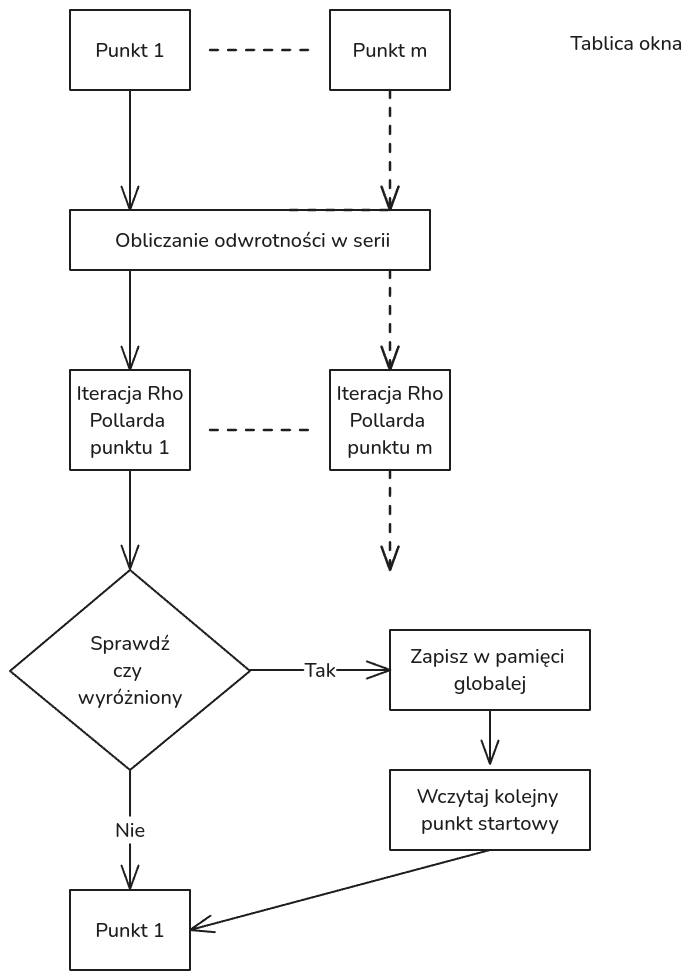
\includegraphics[width=0.8\textwidth]{img/okienkowanie_3.png}
    \caption{Schemat działania pojedynczego kroku w pętli}
    \label{fig:windowing}
\end{figure}

\subsection{Tail effect}
Tail Effect to zjawisko, które polega na nierównomiernym obciążeniu wątków na GPU.
W przypadku równoległej wersji algorytmu Rho Pollard'a, to zjawisko jest szczególnie widoczne,
ze względu na losowość funkcji błądzenia po krzywej.
Wątki znajdują punkty wyróżnione w różnym, losowym czasie.
\par
Po znalezieniu punktu wyróżnionego, wątek musi zaczekać, na zakończenie pracy wszystkich
pozostałych wątków w ramach jednego bloku.
To powoduje, że tylko przez krótki czas są wykorzystywane wszystkie zasoby GPU.
\par
Jednym ze sposobów na zmniejszenie tego efektu, jest wydłużenie czasu pracy każdego z wątków poprzez zwiększenie ilości punktów wyróżnionych,
które musi znaleźć. Dzięki temu spada prawdopodobieństwo, że zakończy on swoją pracę znacznie wcześniej niż pozostałe wątki w bloku.
Zastosowanie metody z oknem, opisanej w poprzedniej sekcji, pozwala na znacznie lepszą utylizację zasobów przez większość
czasu obliczeń.
\par
Rys \ref{fig:tail_effect_1} oraz \ref{fig:tail_effect_3} przedstawiają czas pracy każdego z wątków w bloku, w trakcie jednej fali obliczeń.
W trakcie testu, każdy z wątków poszukiwał punktów wyróżnionych z 17 zerami na końcu współrzędnej $x$. Widoczne jest
znaczne lepsze wykorzystanie zasobów GPU w przypadku, gdy każdy z wątków musi znaleźć 3 punkty wyróżnione przed zakończeniem pracy.
Zmniejsza to wpływ anomalii, gdy punkt wyróżniony jest znajdowany znacznie wcześniej lub później niż wynika z wartości oczekiwanej.

% wykres
\begin{figure}[H]
    \centering
    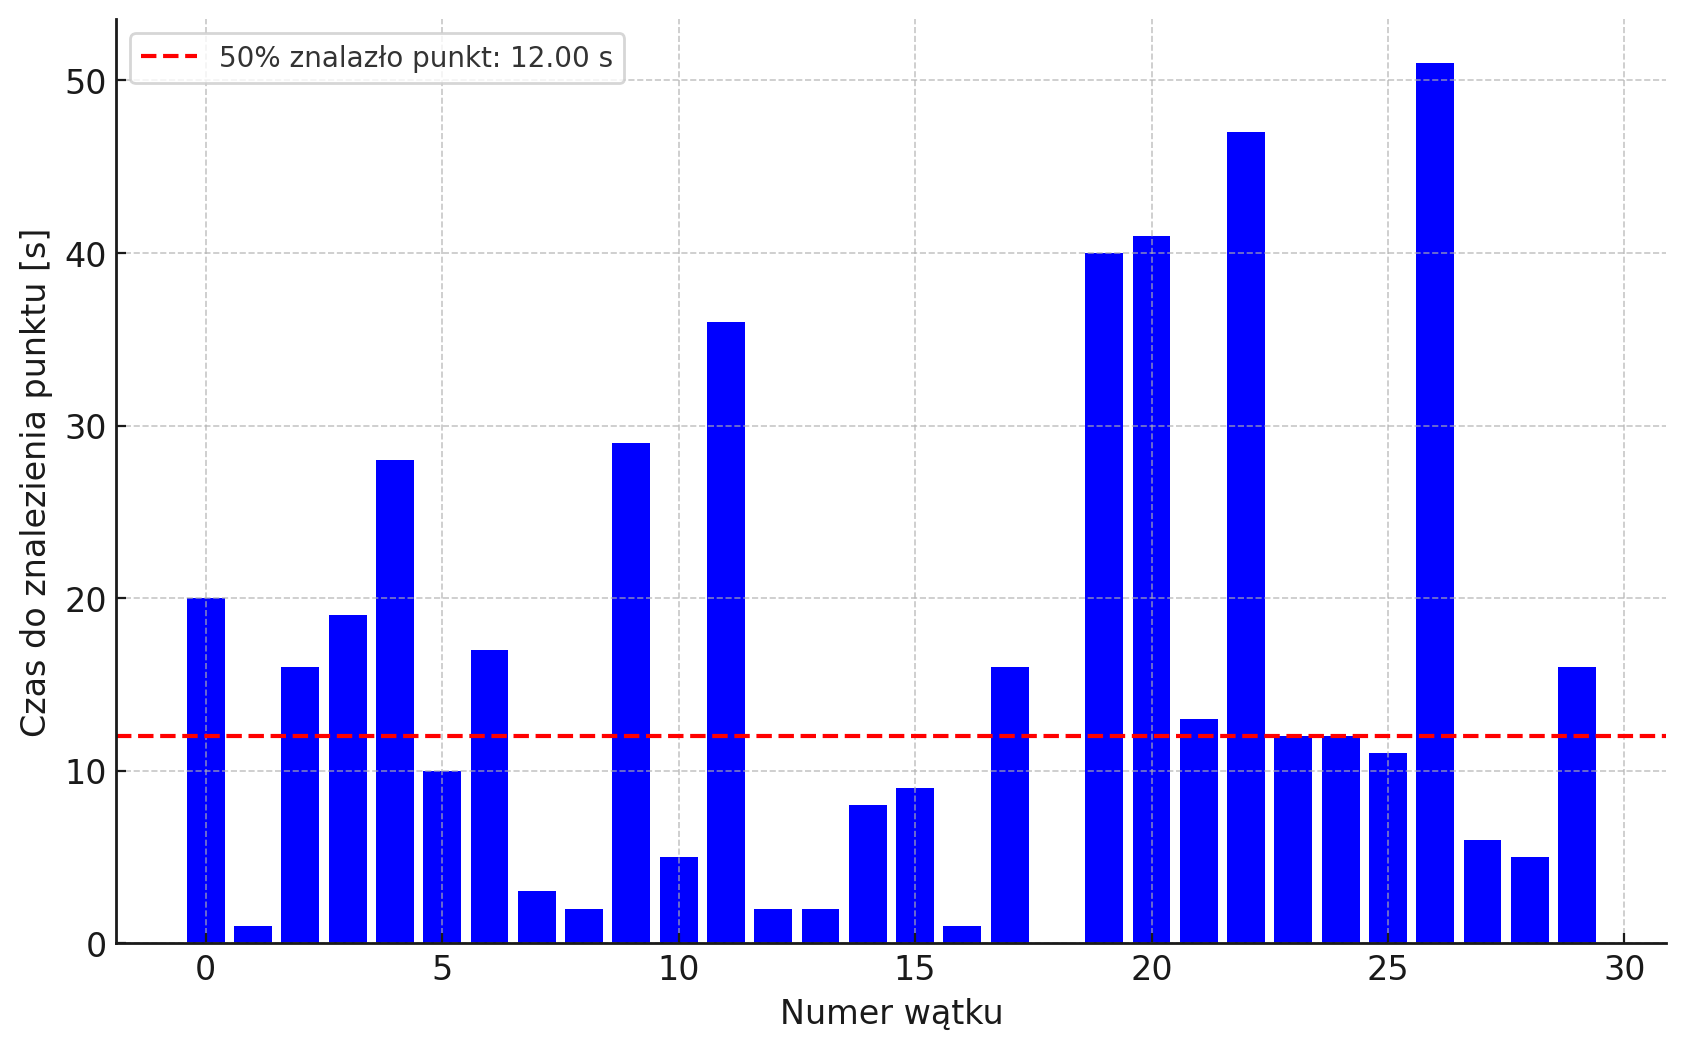
\includegraphics[width=1\textwidth]{img/tailing_effect_single_17.png}
    \caption{Tail effect widoczny na małej grupie wątków. Wątki kończą pracę po znalezieniu jednego punktu wyróżnionego.
        Większość czasu obliczeń, jest wykorzystywana tylko przez małą liczbę wątków.}
    \label{fig:tail_effect_1}
\end{figure}

% wykres
\begin{figure}[H]
    \centering
    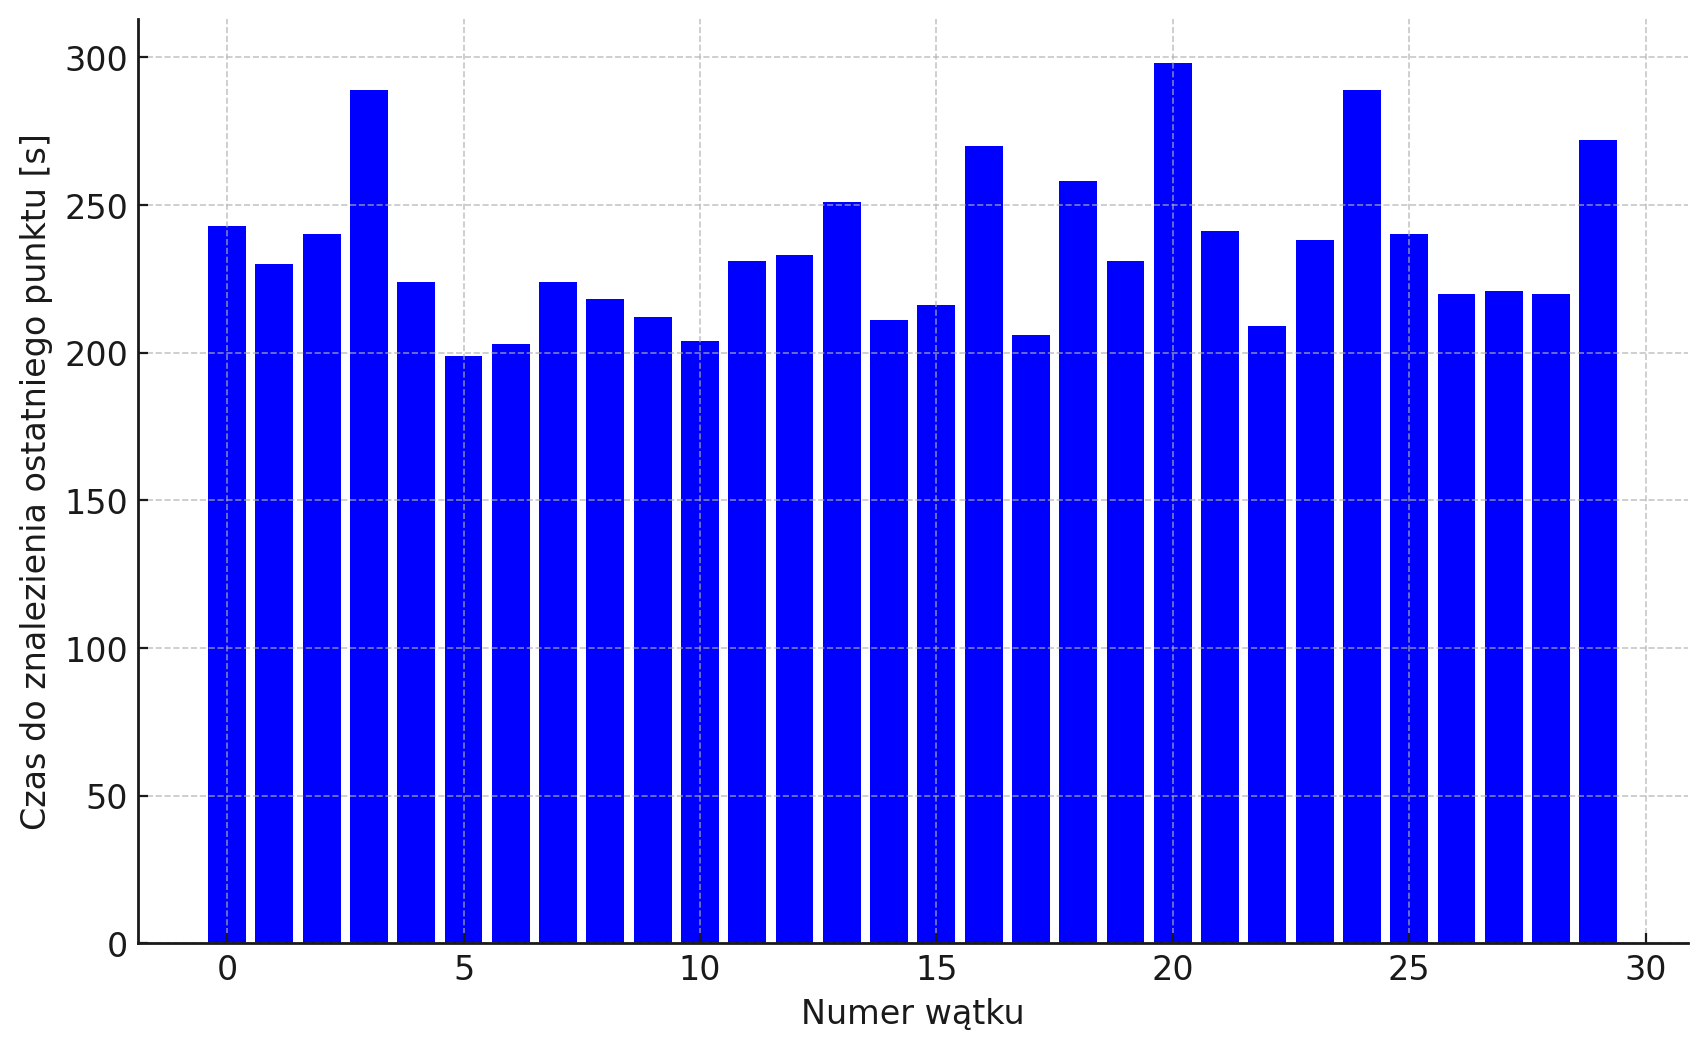
\includegraphics[width=1\textwidth]{img/tailing_effect_3_17.png}
    \caption{Tail effect widoczny na małej grupie wątków. Wątki kończą pracę po znalezieniu 3 punktów wyróżnionych.
        Widoczne jest znacznie lepsze wykorzystanie zasobów GPU, przez większość czasu obliczeń.}
    \label{fig:tail_effect_3}
\end{figure}

\par
Aby jeszcze bardziej zniwelować efekt, zastosowałem specjalną flagę w pamięci współdzielonej, która pozwala zakończyć obliczenia wszystkich wątków w bloku,
po tym, jak pierwszy z nich znajdzie wszystkie punkty wyróżnione. Pozwala to zwolnić miejsce na kolejny blok
i pozwolić na załadowanie nowych danych do obliczeń, gdy tylko poziom wykorzystania zasobów zacznie spadać.
Karty graficzne z architekturą Turing,
pozwalają na kolejkowanie wielu uruchomień kernel'a wykorzystując mechanizm strumieni CUDA.
Dzięki wykorzystaniu strumieni, scheduler CUDA
może uruchamiać kolejne bloki obliczeń z kolejki zadań, gdy tylko
zwolni się miejsce na kolejny blok, zamiast czekać ze startem na zakończenie poprzedniego kernel'a \cite{cuda}.
\par
Rys \ref{fig:tail_effect_3} przedstawia wykres sumy znalezionych punków od czasu przy uruchomieniu dwóch kernel'i w oddzielnych strumieniach.
Widoczne jest przejmowanie przez strumień Stream 2 wolnych zasobów, zwalnianych przez Stream 1.
Wypłaszczenie krzywej sumy punktów pod koniec pracy każdego ze strumieni, jest
efektem ogona, spowodowanym przez nierównomierny czas pracy na poziomie bloków.
Jednak dopóki jest zapewniona zastępowalność bloków na SM, efekt nie wpływa na wydajność obliczeń.



% wykres
\begin{figure}[H]
    \centering
    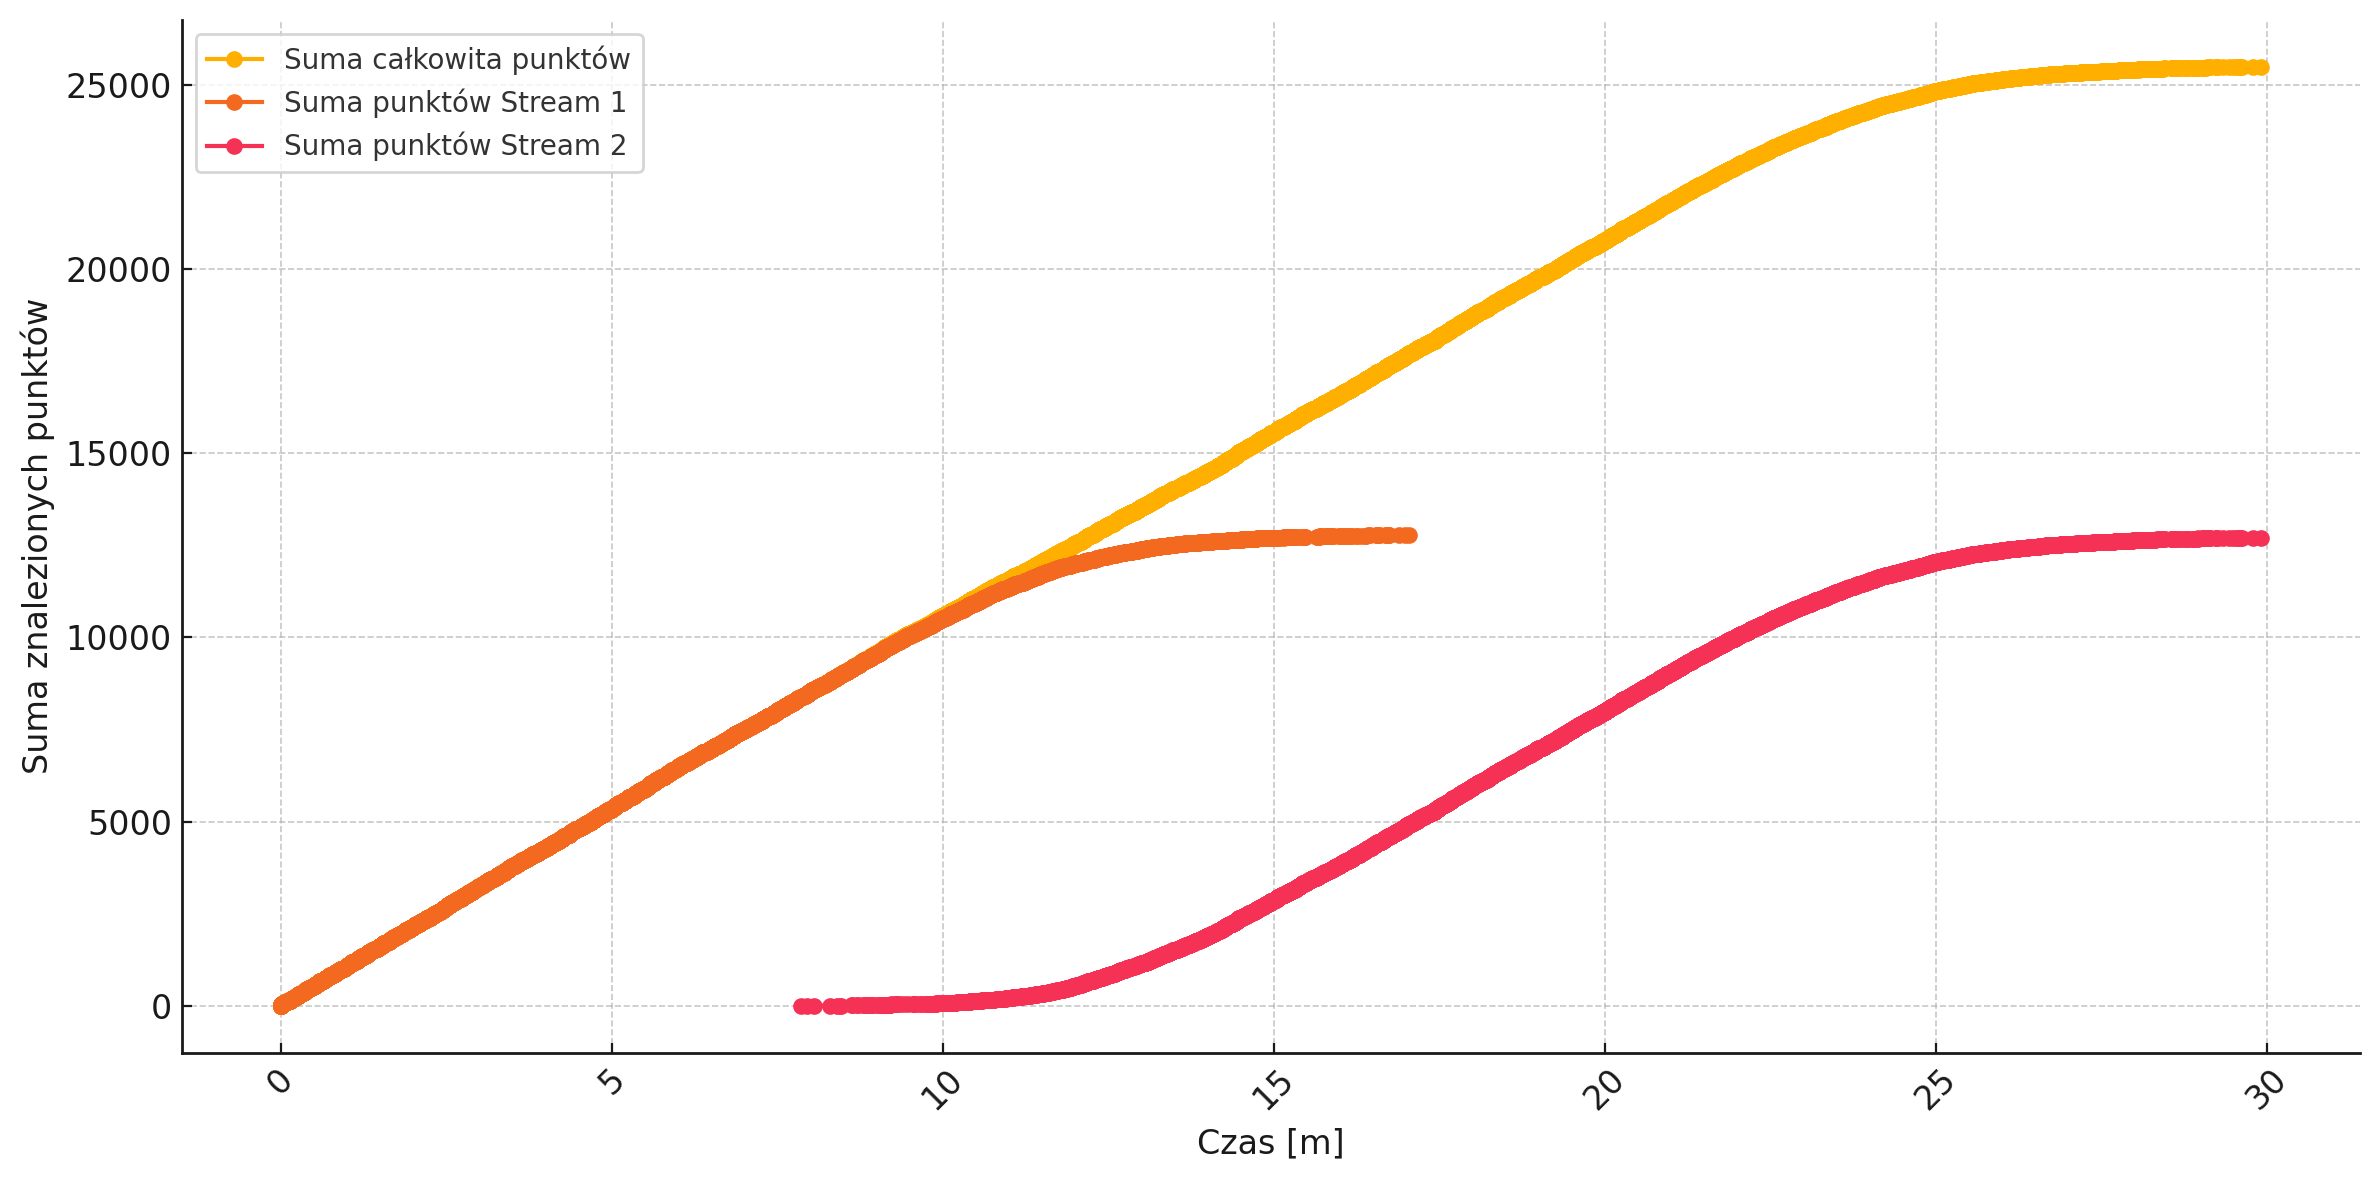
\includegraphics[width=1\textwidth]{img/streams.png}
    \caption{Suma znalezionych punktów wyróżnionych z podziałem na strumienie,
        gdzie każdy z wątków szukał 10 punktów wyróżnionych z 22 zerami na końcu współrzędnej $x$.
        Zastosowano flagę kończenia obliczeń wszystkich wątków w bloku.
        Widoczne jest przejmowanie przez strumień Stream 2 wolnych zasobów, zwalnianych przez Stream 1.
    }
    \label{fig:tail_effect_3}
\end{figure}

\subsection{Program serwera}
Główny cel serwera centralnego w równoległej wersji algorytmu Rho Pollard'a, sprowadza się do
przechowywania obliczonych punktów wyróżnionych oraz poszukiwania wśród nich kolizji.
W mojej implementacji, jego zadania zostały rozszerzone o generowanie punktów startowych
oraz wstępną generację punktów niezbędnych do spaceru losowego w wersji \textit{addition walk}.
\par
Na samym początku działania systemu, serwer startuje odpowiednią ilość
klientów, poprzez uruchamianie w osobnych wątkach funkcji \textit{GPUWorker},
w ilości na tyle dużej, aby wysycić zasoby GPU.
Ponieważ kod działający na GPU został skompilowany z flagą dla kompilatora NVCC \textit{--default-stream per-thread},
każdy z klientów działających w osobnym wątku, tworzy własny strumień CUDA, co pozwala na ich kolejkowanie uruchomionych kernel'i po stronie GPU.
\par
Klienci komunikuje się z serwerem za pomocą dwóch asynchronicznych kolejek FIFO.
Pierwsza z nich służy do przekazywania punktów startowych z serwera do klientów, a druga do przekazywania
znalezionych punktów wyróżnionych przez klientów do serwera. Taka centralizacja
generowania punktów startowych, wynika z problemów z bibliotekami SageMath,
podczas uruchamiania ich kodu w wielu wątkach jednocześnie.
Do uruchamiania skompilowanego kodu dla GPU, wykorzystałem
bibliotekę \textit{Ctypes}, która umożliwia wywoływanie funkcji napisanych w języku C z poziomu Pythona.
\par
Serwer w celu przechowywania punktów otrzymanych od klientów, wykorzystuje
zwykły słownik dostępny w języku Python, który jest odpowiednikiem hash-mapy.
Punkty są przechowywane w formie: \textit{(x,y): seed}, gdzie \textit{seed} oznacza
ziarno z jakiego został wygenerowany punkt startowy, który doprowadził do znalezienia punktu wyróżnionego.
Dzięki temu, w razie kolizji, serwer jest w stanie odtworzyć punkt startowy, a następnie wykonać cały spacer losowy, który doprowadził do danego punktu.
Jest to szczególnie istotne, ponieważ po stronie GPU nie są zliczane parametry $a$ oraz $b$ niezbędne do obliczenia
logarytmu dyskretnego

\subsubsection{Generacja punktów startowych}

Początkowo punkty startowe były generowane za pomocą funkcji skrótu MD5 z operacją
modulo rzędu ciała, jednak bardziej wydajnym podejściem okazało się wykorzystanie
pakietu \texttt{random} z biblioteki standardowej języka Python. Pakiet ten
zapewnia wystarczającą losowość dla tego zastosowania, co umożliwia szybszą
i efektywną generację punktów.

Proces generacji punktów startowych odbywa się wyłącznie po stronie serwera.
Wygenerowane punkty, wraz z odpowiadającymi im ziarnami (\textit{seed}), są
przekazywane do klienta. Jeśli jednak wygenerowany punkt startowy spełnia od razu
kryteria punktu wyróżnionego, zostaje przekazany bezpośrednio do puli punktów
wyróżnionych i nie zajmuje miejsca wśród punktów startowych. Dzięki temu zasoby
są lepiej wykorzystywane, a redundancja w obliczeniach jest zredukowana.

Przykładowy kod generacji punktów w języku Python:

\begin{lstlisting}[language=Python, caption=Generacja punktów startowych]
def generate_starting_points(instances, zeros_count):
    distinguish_points = []
    starting_points = []
    i = 0
    while i < instances:
        seed = int.from_bytes(random.randbytes(10), "big") % curve_order
        A = P * seed
        x = int(A[0])
        y = int(A[1])
        if not is_distinguish(x, zeros_count):
            i += 1
            starting_points.append((x, y, seed))
        else:
            distinguish_points.append((x, y, seed))
    return starting_points, distinguish_points
\end{lstlisting}

\subsubsection{Kolizje}

W przypadku wykrycia kolizji serwer pobiera ziarna obu punktów i odtwarza
kolejne kroki algorytmu, które doprowadziły do ich znalezienia. W tym procesie
serwer oblicza wielokrotności punktów $P$ oraz $Q$, co pozwala na określenie
logarytmu dyskretnego. W rzadkich przypadkach, gdy obliczenie odwrotności modularnej
jest niemożliwe (np. mianownik wynosi $0$ w algorytmie Rho Pollard'a), obliczenie
logarytmu dyskretnego może się nie powieść.

Jeżeli jednak obliczenia zakończą się sukcesem, serwer wyznacza logarytm
dyskretny i wysyła sygnał do zakończenia dalszych obliczeń. Wynik końcowy jest
następnie przekazywany na standardowe wyjście (\texttt{stdout}).

Przykładowa implementacja funkcji obliczającej współczynniki $a$ i $b$ w Pythonie:

\begin{lstlisting}[language=Python, caption=Obliczanie współczynników $a$ i $b$]
def calculate_ab(seed, precomputed_points: list[PrecomputedPoint]):
    a_sum = seed
    b_sum = 0
    W = P * seed
    while not is_distinguish(W[0], ZEROS_COUNT):
        precomp_index = map_to_index(W[0])
        precomputed = precomputed_points[precomp_index]
        R = precomputed.point
        a_sum = a_sum + precomputed.a
        b_sum = b_sum + precomputed.b
        W = W + R
    a_sum = a_sum % curve_order
    b_sum = b_sum % curve_order
    return (a_sum, b_sum)
\end{lstlisting}

Funkcja \texttt{calculate\_ab} przyjmuje ziarno oraz listę wcześniej
obliczonych punktów. Kolejne wielokrotności punktów $P$ i $Q$ są sumowane wraz
z ich współczynnikami $a$ i $b$, aż do napotkania punktu wyróżnionego. Wynikowe
wartości są redukowane modulo rząd krzywej i zwracane jako współczynniki, które
umożliwiają wyznaczenie logarytmu dyskretnego.

\subsection{Logowanie}

W celu monitorowania wydajności systemu oraz postępu obliczeń, zarówno w kodzie
klienta, jak i serwera, zaimplementowano mechanizm logowania. CUDA umożliwia
wypisywanie informacji na standardowe wyjście (\texttt{stdout}) za pomocą funkcji
\texttt{printf}, analogicznie jak w standardowym języku C. W głównym kernel'u kodu
można aktywować logowanie, ustawiając odpowiednią flagę za pomocą dyrektywy
\texttt{\#define logging}.

Logowane dane w kernel'u obejmują:
\begin{itemize}
    \item czas znalezienia punktu wyróżnionego,
    \item numer wątku,
    \item numer bloku,
    \item numer strumienia.
\end{itemize}

Przykładowy fragment logów generowanych przez kernel:
\begin{verbatim}
Wed Sep 18 01:14:33 AM CEST 2024 STREAM 0, instance: 8253 found distinguish point 0
Wed Sep 18 01:14:33 AM CEST 2024 STREAM 0, instance: 28320 found distinguish point 0
Wed Sep 18 01:14:33 AM CEST 2024 STREAM 0, instance: 19113 found distinguish point 0
Wed Sep 18 01:14:33 AM CEST 2024 STREAM 0, instance: 28214 found distinguish point 0
Wed Sep 18 01:14:33 AM CEST 2024 STREAM 0, instance: 24343 found distinguish point 0
\end{verbatim}

Dodatkowo, serwer po każdorazowym otrzymaniu danych od zakończonych obliczeń
w kernel'u wypisuje informacje o łącznej liczbie punktów wyróżnionych, które
zgromadził do tej pory. Przykładowe logi generowane przez serwer:
\begin{verbatim}
Wed Sep 18 07:13:45 PM CEST 2024 Got new distinguish points
Wed Sep 18 07:13:45 PM CEST 2024 Currently have 941239
Wed Sep 18 07:13:45 PM CEST 2024 GPU worker 0 got task
Wed Sep 18 07:13:45 PM CEST 2024 Got 957733 points
\end{verbatim}

Mechanizm logowania umożliwił dokładniejszą analizę wykorzystania zasobów GPU oraz
optymalne dostosowanie liczby wątków i bloków do struktury sprzętowej. Dane logowane
były zapisywane do pliku, co pozwoliło na dalsze przetwarzanie, takie jak mierzenie
wydajności i wizualizację wyników w formie wykresów. Wizualizacje te przedstawiają
między innymi sumę znalezionych punktów od czasu,
co pozwoliło oszacować wydajność projektu.

\section{Wyniki}
\subsection{Testy implementacji}

Głównym celem pracy było znalezienie rozwiązania problemu logarytmu dyskretnego
dla krzywej ECCp79 z Certicom Challenge w możliwie najkrótszym czasie. Mimo że
rozmiar krzywej jest stosunkowo niewielki, a współczesny sprzęt znacznie
wydajniejszy od tego dostępnego w momencie pierwszych prób złamania tej krzywej,
obliczenie rozwiązania wciąż zajmuje czas liczony w godzinach.

Ze względu na czasochłonność pełnych obliczeń, niezbędne było przeprowadzenie
testów implementacji na mniejszych, uproszczonych problemach, które pozwoliłyby
na szybszą weryfikację poprawności algorytmu i jego działania. Testy te były
niezbędnym krokiem przed przystąpieniem do pełnoprawnych prób rozwiązania
problemu logarytmu dyskretnego dla krzywej ECCp79. Pozwoliły one na upewnienie się,
że implementacja działa poprawnie oraz spełnia wszystkie założenia teoretyczne.

W tym celu wykorzystano środowiska PyTest oraz SageMath do przeprowadzenia testów
funkcjonalnych, weryfikujących poprawność operacji na krzywych eliptycznych
oraz pierwszych kroków algorytmu Rho Pollarda.

Testy obejmowały następujące aspekty:
\begin{itemize}
    \item Poprawność dodawania punktów na krzywej eliptycznej:
          Wyniki obliczeń programu klienta były porównywane z wynikami uzyskanymi
          w SageMath.
    \item Weryfikacja pierwszych kilkuset iteracji algorytmu Rho Pollarda:
          Sprawdzano zgodność wyników generowanych przez implementację z oczekiwanymi
          wartościami teoretycznymi.
    \item Sprawdzenie integralności przesyłanych danych pomiędzy serwerem a
          klientem: Testowano, czy format danych oraz zawartość są poprawnie przetwarzane
          na styku kodu Python'a oraz CUDA.
\end{itemize}

Wszystkie testy zostały pomyślnie zaliczone w obecnej wersji programu, co
potwierdza poprawność implementacji oraz zgodność wyników z teoretycznymi
oczekiwaniami.

\subsection{Wydajność}

W celu oceny wydajności implementacji program był wielokrotnie uruchamiany z
włączonym pełnym logowaniem każdego znalezionego punktu wyróżnionego. Wydajność
mierzono na podstawie przyrostu liczby znalezionych punktów w czasie, co pozwalało
na oszacowanie liczby iteracji dodawania punktów na sekundę.

Testy przeprowadzono przy założeniu, że punkt wyróżniony spełnia warunek 20
najmłodszych bitów współrzędnej $x$ równych $0$ w reprezentacji bitowej.
Sprawdzano sumę znalezionych punktów wyróżnionych w różnych odstępach czasu:
po 1 minucie oraz 5 minutach.

\begin{table}[h!]
    \centering
    \caption{Wyniki testów wydajności}
    \begin{tabular}{|c|c|c|}
        \hline
        \textbf{Czas testu} & \textbf{Liczba znalezionych punktów} &
        \textbf{Średnia liczba iteracji/s}                                \\ \hline
        1 minuta            & 5274                                 & 87.9 \\ \hline
        5 minut             & 26310                                & 87.7 \\ \hline
        % 10 minut            & <liczba punktów>                     & <wynik> \\ \hline
    \end{tabular}
    \label{tab:performance}
\end{table}

Na podstawie wyników testów oszacowano liczbę operacji dodawania punktów na
sekundę w algorytmie Rho Pollarda. Prawdopodobieństwo znalezienia punktu wyróżnionego,
gdy 20 najmłodszych bitów współrzędnej $x$ wynosi $0$, można określić jako
$$
    P = 2^{-20}.
$$

Średnia liczba iteracji potrzebna do znalezienia punktu wyróżnionego wynosi
więc:
$$
    \text{Średnia liczba iteracji} = \frac{1}{P} = 2^{20}.
$$

Na podstawie wyników testów, oszacowano, że implementacja osiąga wydajność na
poziomie 87,7 milionów operacji dodawania punktów na sekundę.

\subsection{Rozwiązanie ECDLP dla krzywej ECCp79}

Najważniejszym wyznacznikiem osiągnięcia założonego celu tej pracy było
znalezienie poprawnego rozwiązania ECDLP dla krzywej z challenge'u Certicom ECCp79.
Po zweryfikowaniu poprawności implementacji na znacznie mniejszych rozmiarach
krzywych eliptycznych, przystąpiłem do przeprowadzenia obliczeń dla docelowego
problemu. Proces ten wymagał wykonania dużej liczby iteracji algorytmu Rho Pollarda,
a jego wyniki zostały szczegółowo udokumentowane.

\begin{figure}[H]
    \centering
    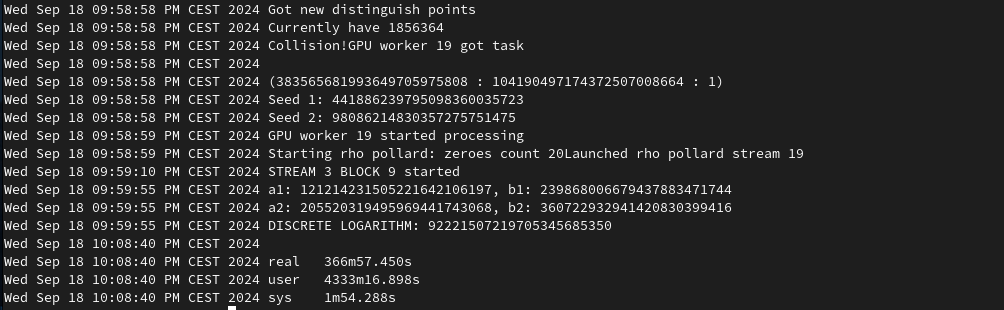
\includegraphics[width=0.8\textwidth]{img/first_attempt.png}
    \caption{Wynik działania programu}
    \label{fig:first_attempt}
\end{figure}

Poniżej przedstawiono wyniki pięciu niezależnych prób obliczenia ECDLP dla
krzywej ECCp79, wskazujące liczbę znalezionych punktów wyróżnionych do momentu
znalezienia kolizji oraz czas trwania obliczeń.

\begin{table}[H]
    \centering
    \caption{Wyniki obliczeń ECDLP dla krzywej ECCp79}
    \label{tab:eccp79_results}
    \begin{tabular}{|c|c|c|}
        \hline
        \textbf{Próba}   & \textbf{Liczba znalezionych punktów} &
        \textbf{Czas trwania obliczeń [s]}                                      \\ \hline
        1                & 1856364                             & 22195.42      \\ \hline
        2                & 791747                              & 9898.74       \\ \hline
        3                & 770077                              & 9329.74       \\ \hline
        4                & 1163047                             & 13681.16      \\ \hline
        5                & 1207014                             & 15001.94      \\ \hline
        \textbf{Średnia} & 1153649                             & 14021.00      \\ \hline
    \end{tabular}
\end{table}



\paragraph{Weryfikacja wyników za pomocą SageMath.}
Aby upewnić się, że uzyskane rozwiązanie ECDLP jest poprawne, przeprowadzono
weryfikację przy użyciu oprogramowania SageMath. Weryfikacja polegała na
podstawieniu uzyskanego wyniku logarytmu dyskretnego do równania punktowego
na krzywej eliptycznej i sprawdzeniu, czy generuje on punkt publiczny
zgodny z założeniami challenge'u Certicom ECCp79.

\begin{figure}[H]
    \centering
    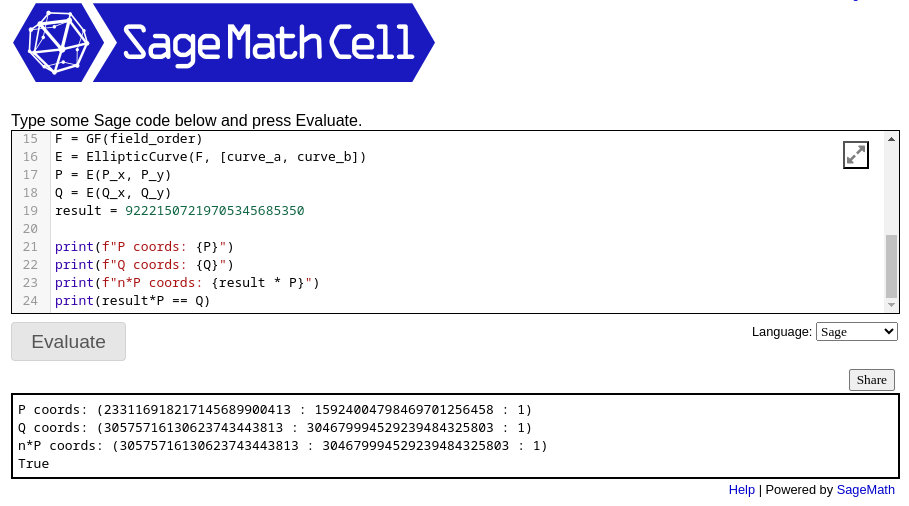
\includegraphics[width=0.8\textwidth]{img/sage_check_full.png}
    \caption{Weryfikacja wyniku w SageMath}
    \label{fig:sage_verification}
\end{figure}

Weryfikacja potwierdziła poprawność uzyskanego wyniku, co dowodzi skuteczności
implementacji oraz poprawności algorytmu w zastosowaniu do krzywej ECCp79.

\paragraph{Podsumowanie wyników.}
Na podstawie powyższych wyników można obliczyć średnią liczbę punktów wyróżnionych
znajdowanych przed wystąpieniem kolizji.
Porównanie wyniku z oczekiwanymi wartościami teoretycznymi, pozwoliło potwierdzić
osiągnięcie odpowiedniej losowości przy obliczaniu kolejnych kroków algorytmu.
Oczekiwaną liczbę punktów do znalezienia kolizji można oszacować na podstawie wzoru:
$$
    E = \frac{\sqrt{\pi \cdot n / 2}}{2^k}
$$
gdzie $n$ to liczność grupy punktów na krzywej eliptycznej, a $k$ to liczba bitów zerowych które decydują
czy dany punkt jest wyróżniony. W przypadku krzywej ECCp79,
dla $n \approx 2^{79}$, oraz punktów wyróżnionych których ostatnie 20 bitów to $0$, oczekiwana liczba
punktów potrzebna do znalezienia kolizji:
$$
    \frac{\sqrt{\pi \cdot 2^{79} / 2}}{2^{20}} = 929262.5811
$$
Uzyskany wynik na poziomie 1153649 jest bliski wartości oczekiwanej. Rozbieżność może wynikać z niewielkiej
liczby przeprowadzonych prób oraz ograniczonej liczby punktów wstępnie obliczonych.
Wydajność obliczeń jest zgodna z wynikami otrzymanymi podczas testów wydajności na ograniczonej liczbie iteracji algorytmu.
Najszybsze znalezienie logarytmu dyskretnego zajeło mniej niż 3 godziny, co jest bardzo zadowalającym wynikiem.
\newpage
\section{Podsumowanie oraz dalsze usprawnienia}

Realizacja pracy pozwoliła mi na zgłębienie zagadnień związanych ze
współczesną kryptografią oraz jej praktyczną implementację. Dodatkowo,
poznałem techniki akceleracji obliczeń z wykorzystaniem GPU. Efekty mojej pracy
uważam za satysfakcjonujące, ponieważ udało się zrealizować wszystkie
założone cele. Obliczenie poprawnego rozwiązania dla wyzwania Certicom,
osiągając wydajność porównywalną z podobnymi pracami, uważam za spory sukces,
biorąc pod uwagę, że była to moja pierwsza styczność z technologią CUDA oraz
kryptografią opartą o krzywe eliptyczne. W pracy pozostaje jednak miejsce na
potencjalne optymalizacje i usprawnienia.

Wykorzystanie lżejszych bibliotek niż pakiet SageMath pozwoliłoby na
łatwiejsze uruchomienie rozwiązania na innych platformach, bez potrzeby
czasochłonnej kompilacji całego pakietu obliczeniowego, którego znaczna
część nie jest wykorzystywana.
Zastosowanie redukcji Barrett'a do operacji dzielenia modulo $p$ pozwoliłoby
jeszcze bardziej zwiększyć wydajność obliczeń na ciele. Ponieważ wszystkie
obliczenia są wykonywane na tych samych parametrach ciała, przeliczenie
specjalnej wartości wymaganej przez tę technikę odbyłoby się tylko raz na
początku obliczeń.

Kolejnym miejscem na potencjalne usprawnienia jest optymalizacja wykorzystania 
rejestrów w kernel'u CUDA. Obecna implementacja ma niewielką liczbę rejestrów,
które musiały być przerzucone przez kompilator do wolniejszej pamięci
globalnej. Prawdopodobnie uważna optymalizacja oraz dokładniejsza analiza z
pomocą profiler'a \textit{NVIDIA Nsight Systems} pozwoliłaby zredukować ilość
"rozlanych" rejestrów, ograniczając narzut związany z niższą
przepustowością pamięci globalnej, oraz zmniejszyć liczbę rozgałęzień w kodzie.

Praca pokazała, że GPU umożliwia osiągnięcie wysokiej wydajności w obliczeniach
kryptograficznych, jednak pomimo rosnącej mocy obliczeniowej oraz wysokiej dostępności
GPU, rozmiar kluczy stosowanych we współczesnej kryptografii nadal zapewnia
odpowiedni poziom bezpieczeństwa. W efekcie złamanie kryptosystemów opartych na
ECC w rozsądnym czasie pozostaje praktycznie niemożliwe.

%--------------------------------------------
% Literatura
%--------------------------------------------
\newpage
\printbibliography
%--------------------------------------------
% Spisy (opcjonalne)
%--------------------------------------------
\newpage

% Wykaz symboli i skrótów.
% Pamiętaj, żeby posortować symbole alfabetycznie
% we własnym zakresie. Ponieważ mało kto używa takiego wykazu, 
% uznałem, że robienie automatycznie sortowanej listy
% na poziomie LaTeXa to za duży overkill. 
% Makro \acronymlist generuje właściwy tytuł sekcji, 
% w zależności od języka.
% Makro \acronym dodaje skrót/symbol to listy, 
% zapewniając podstawowe formatowanie.
% //AB
\vspace{0.8cm}
\acronymlist
\acronym{EiTI}{Wydział Elektroniki i Technik Informacyjnych}
\acronym{PW}{Politechnika Warszawska}
\acronym{FPGA}{Field Programmable Gates Array}
\acronym{CUDA}{Compute Unified Device Architecture}
\acronym{ECC}{Elliptic Curve Cryptography}
\acronym{DLP}{Discrete Logarithm Problem}
\acronym{GF}{Galois Field (ciało skończone)}

\listoffigures              % Spis obrazków. 
\vspace{1cm}                % vertical space
\listoftables               % Spis tabel. 
\vspace{1cm}               % vertical space
\lstlistoflistings 		% Spis wydruków
\vspace{1cm}                % vertical space
\listofappendices           % Spis załączników

% Załączniki

%\newpage
%\appendix{Nazwa załącznika 1}
%\lipsum[1]
%
%\newpage
%\appendix{Nazwa załącznika 2}
%\lipsum[1]
% Załączniki

%\newpage

% jesli sa w~Zalacznikach tabele, rysunki, tak na szybko.. i~wylaczyc \listofappendices
%\section*{Załącznik I. Wykaz komend AT czujnika parkowania AN-101D firmy Shenzhen Winext Technology}
%%\appendix{Wykaz komend AT czujnika parkowania AN-101D firmy Shenzhen Winext Technology.}
%\setcounter{section}{1}
%\renewcommand\thetable{I.\arabic{table}}
%\input{tex/zal-1-komendy-at}
%
%\newpage
%\section*{Załącznik II. Ramki komunikacyjne czujnika parkowania AN-101D firmy Shenzhen Winext Technology}
%%\appendix{Ramki komunikacyjne czujnika parkowania AN-101D firmy Shenzhen Winext Technology.}
%\renewcommand\thefigure{II.\arabic{figure}}
%\input{tex/zal-2-ramki-komunikacyjne}




\end{document} % Dobranoc. 

